\documentclass[11pt]{iopart}
\usepackage[english]{babel}
\pdfoutput=1
%\usepackage{amsmath}
\usepackage{wasysym}
\usepackage{booktabs}
\usepackage{amssymb}
\usepackage{amsbsy}
\usepackage{verbatim}
\usepackage{graphicx}
\usepackage{epstopdf}
\usepackage{color}
\usepackage{sidecap}
\usepackage{bm}% bold math
\usepackage{tikz}
%\usepackage[backend=bibtex]{biblatex}

\usepackage[colorlinks,bookmarks=false,citecolor=blue,linkcolor=red,urlcolor=blue]{hyperref}

\newcommand*\circled[1]{\tikz[baseline=(char.base)]{
            \node[shape=circle,draw,inner sep=2pt] (char) {#1};}}


\usepackage{cite}

%
% WARNING !!!!
% 
% iopart.cls definition of \tableofcontents overwrites the
% short title printed every page. 
% The following redefinition of \tableofcontents fixes the
% the problem. 

\catcode`@=11 % If we need private TeX macros
\renewcommand\tableofcontents{%
  \section*{\contentsname}%
  \@starttoc{toc}%
}
\catcode`@=12% '@' is no more a character
\newcommand{\bra}[1]{\langle\left.{#1}\right|}
\newcommand{\ket}[1]{\left|{#1}\right.\rangle}


\def\be{\begin{equation}}
\def\ee{\end{equation}}
\def\u{\uparrow}
\def\d{\downarrow}
\def\nm{\newmoon}
\def\fm{\fullmoon}
\def\T{\rule{0pt}{.6cm}}
\def\B{\rule[-.4cm]{0pt}{0pt}}

\begin{document}

\setlength{\parindent}{0pt}


\title{The quench action approach for integrable models: A Monte Carlo implementation}

\author{Authors}
%\address{$^1$ International School for Advanced Studies (SISSA),
%Via Bonomea 265, 34136, Trieste, Italy,
%INFN, Sezione di Trieste}


\date{\today}



%%%%%%%%%%%%%%%%%%%%%%%%%%%%%%%%%%%%%%%%%%%%%%%%%%%%%%%%%%%%%%%%%%%%%%%%%%
\begin{abstract} 


fdasfa
\end{abstract}

\maketitle

%%%%%%%%%%%%%%%%% INTRODUCTION %%%%%%%%%%%%%%%%%%%%%
\section{Introduction}
\label{intro}

Understanding the out-of-equilibrium dynamics in {\it isolated} quantum 
many-body systems is one of the most intriguing research topics in 
contemporary physics~\cite{polkovnikov-2011}, both theoretically and 
experimentally. The most common out-of-equilibrium protocol is the {\it 
quantum quench} in which a system is initially prepared in an eigenstate 
$|\Psi_0\rangle$ of a many-body hamiltonian ${\mathcal H}$. Then a global 
parameter of the hamiltonian is suddenly changed, and the system is let 
to evolve unitarily under a new Hamiltonian ${\mathcal H}'$. 

While there is now compelling evidence that at long times after the 
quench a steady state arises, its nature is still highly debated. 
In the thermodynamic limit it is natural to expect that the steady-state 
value of any local observable ${\mathcal O}$ is given by the so-called 
diagonal ensemble as 
%
\begin{equation}
\label{d-ensemble}
\langle{\mathcal O}\rangle_{DE}=\sum\limits_{\lambda}|\langle\Psi_0|\lambda
\rangle|^2\langle\lambda|{\mathcal O}|\lambda\rangle,
\end{equation}
%
where the sum is over the eigenstates $|\lambda\rangle$ of the post-quench 
final hamiltonian ${\mathcal H}'$. For generic, i.e., non-integrable, models 
the Eigenstate Thermalization Hypothesis ensures that the ensemble~\eref{d-ensemble} 
becomes equivalent to the Gibbs (thermal) ensemble, implying 
%
\begin{equation}
\langle{\mathcal O}\rangle_{DE}=\langle{\mathcal O}\rangle_{Gibbs}\equiv
\frac{1}{Z}\Tr({\mathcal O}\rho^{Gibbs}),\quad\textrm{with}\quad\rho^{Gibbs}
=e^{-\beta{\mathcal H}'},
\end{equation}
%
where $\beta$ is the inverse temperature of the system and $Z$ a normalization 
factor. For one-dimensional integrable models, the presence of local or quasi-local 
integrals of motion strongly affects the dynamics, preventing the onset of 
thermal behavior at long times. It has been suggested that the long time 
steady state behavior is described by the so-called Generalized Gibbs 
ensemble as 
%
\begin{equation}
\langle{\mathcal O}\rangle_{GGE}=\frac{1}{Z}\Tr({\mathcal O}\rho^{GGE}), 
\quad\textrm{with}\quad\rho^{GGE}\equiv\frac{1}{Z}\exp\Big(-\sum_j\beta_jQ_j\Big)
\end{equation}
%
We show that it is possible to numerically simulate the Quench Action approach 
combining Monte Carlo methods and Bethe ansatz techniques. 

We focus on the situation in which the pre-quench initial state is the Neel 
state or the Majumdar-Ghosh state. 

We investigate the importance of the zero-momentum strings in the Quench Action. 

Without zero-momentum strings the overlap saturation rules are not valid, 
i.e., in finite size systems the vast majority of the eigenstates contain 
zero momentum strings. 

The details on the eigenstates counting depend on the pre-quench initial state. 

However, we show that one can restrict to the set of non-zero momentum strings. 
The fact that one neglects zero-momentum strings gives rise only to scaling 
corrections. 

We also investigate the validity of the Bethe-Takahashi approximation for the 
calculation of the overlap. 

It is useful to rewrite~\eref{d-ensemble} as 
%
\begin{equation}
\label{qa-prob}
\langle{\mathcal O}\rangle=\sum\limits_{\alpha}\rho^{DE}(\alpha)
\langle\alpha|{\mathcal O}|\alpha\rangle,\quad\textrm{with}\quad 
\rho^{DE}(\alpha)=\exp(-2\Re{\mathcal E}(\alpha)).
\end{equation}
%
Here $\rho^{DE}(\alpha)$ is a diagonal ensemble density matrix, and ${\mathcal E}(\alpha)
\equiv-\log\langle\alpha|\Psi_0\rangle$, with $\Re$ denoting the real part. 

The N\'eel state is defined as 
%
\begin{equation}
\label{neel}
|N\rangle\equiv\frac{1}{\sqrt{2}}\big(|N_1\rangle
+|N_2\rangle\big), 
\end{equation}
%
with $|N_1\rangle\equiv |\uparrow\downarrow\rangle^{\otimes L/2}$, and $|N_2\rangle\equiv 
|\downarrow\uparrow\rangle^{\otimes L/2}$. Note that $|N_1\rangle=\hat T|N_2\rangle$, 
with $\hat T$ the one-site shift operator. 


The Majumdar-Ghosh state $|MG\rangle$ is defined as 
%
\begin{equation}
\label{mg}
|MG\rangle\equiv \Big(\frac{|\uparrow\downarrow\rangle-|\downarrow\uparrow\rangle}
{\sqrt{2}}\Big)^{\otimes L/2}. 
\end{equation}
%

%%%%%%%%%%%%%%%%%%%%%%% BETHE ANSATZ FOR THE XXX CHAIN %%%%%%%%%%%%%%%%%%%%%%%%%%
\section{Bethe ansatz solution of the Heisenberg ($XXX$) spin chain}
\label{sec:1}

Here we review some Bethe ansatz results for the spin-$\frac{1}{2}$ Heisenberg 
($XXX$) chain. Specifically, in section~\ref{sec:1.1} we introduce the model. 
Its eigenstates (Bethe states) and the Bethe equations are discussed in 
section~\ref{sec:1.2}. Section~\ref{sec:1.3} focuses on the string hypothesis 
and the so-called Bethe-Gaudin-Takahashi (BGT) equations. The form of the 
BGT equations in the thermodynamic limit is discussed in section~\ref{sec:1.4}. 
Finally, in section~\ref{sec:1.5} we provide the exact formulas for the 
local conserved charges of the model. 


%%%%%%%%%%%%%%%%%%%%%%%%%%%%%%%%%%%%%%%%%%%%%%%%%%%%%%%%%%%%%%%%%%%%%%%%%%%
\subsection{The spin-$\frac{1}{2}$ Heisenberg chain}
\label{sec:1.1}

The spin-$\frac{1}{2}$ isotropic Heisenberg chain ($XXX$ chain) with $L$ sites 
is defined by the Hamiltonian 
%
\begin{equation}
\label{xxx-ham}
{\mathcal H}\equiv J\sum\limits_{i=1}^L\left[\frac{1}{2}(S_i^+S^-_{i+1} 
+S_i^{-}S_{i+1}^+)+S_i^zS_{i+1}^z-\frac{1}{4}\right],  
\end{equation}
%
where $S^{\pm}_i\equiv (\sigma_i^x\pm i\sigma_i^y)/2$ are spin operators acting on the 
site $i$, $S_i^z\equiv\sigma_i^z/2$, and $\sigma^{x,y,z}_i$ the Pauli matrices. Here we 
fix $J=1$ and use periodic boundary conditions, identifying sites $L+1$ and $1$. The 
total magnetization $S_{T}^z\equiv\sum_iS_i^z=L/2-M$, with $M$ number of down spins 
(particles), commutes with~\eref{xxx-ham}, and it is used to label its eigenstates. 


%%%%%%%%%%%%%%%%%%%%%%%%%%%%%%%%%%%%%%%%%%%%%%%%%%%%%%%%%%%%%%%%%%%%%%%%%%%
\subsection{Bethe equations and wavefunctions}
\label{sec:1.2}


In the Bethe ansatz framework~\cite{bethe-1931,taka-book} the generic eigenstate 
of~\eref{xxx-ham} (Bethe state) in the sector with $M$ particles can be written as 
%
\begin{equation}
\label{ba-eig}
|\Psi_M\rangle=\sum\limits_{1\le x_1<x_2<\dots<x_M\le L}A_M(x_1,x_2,
\dots,x_M)|x_1,x_2,\dots,x_M\rangle,
\end{equation}
%
where the sum is over the positions $\{x_i\}_{i=1}^M$ of the particles, and $A_M(x_1,
x_2,\dots,x_M)$ is the eigenstate amplitude corresponding to the particles 
being at positions $x_1,x_2,\dots, x_M$. The amplitude $A_M(x_1,x_2,\dots, x_M)$ is 
given as 
%
\begin{equation}
\label{ba_amp}
A_M(x_1,x_2,\dots,x_M)\equiv\sum\limits_{\sigma\in S_M}\exp\Big[i
\sum\limits_{j=1}^Mk_{\sigma_j}x_j+i\sum\limits_{i<j}\theta_{\sigma_i,\sigma_j}
\Big], 
\end{equation}
%
where the outermost summation is over the permutations $S_M$ of the so-called 
quasi-momenta $\{k_\alpha\}_{\alpha=1}^M$. The two-particle scattering phases 
$\theta_{\alpha,\beta}$ are defined as 
%
\begin{equation}
\label{s_phases}
\theta_{\alpha,\beta}\equiv \frac{1}{2i}\log\Big[-\frac{e^{ik_\alpha+ik_\beta}-
2e^{ik_\alpha}+1}{e^{ik_\alpha+ik_\beta}-2e^{ik_\beta}+1}\Big].
\end{equation}
%
The eigenenergy associated with the eigenstate~\eref{ba-eig} is  
%
\begin{equation}
\label{ba-ener}
E=\sum\limits_{\alpha=1}^M(\cos(k_\alpha)-1). 
\end{equation}
%
The quasi-momenta $k_\alpha$ are obtained by solving the so-called Bethe 
equations~\cite{bethe-1931}
%
\begin{equation}
\label{ba-eq}
e^{ik_\alpha L}=\prod\limits^M_{\beta\ne\alpha}\Big[-\frac{1-2e^{
ik_\alpha}-e^{ik_\alpha+ik_\beta}}{1-2e^{ik_\beta}-e^{ik_\alpha+
ik_\beta}}\Big].
\end{equation}
%
It is useful to  introduce the rapidities $\{\lambda_\alpha\}_{\alpha=1}^M$ as 
%
\begin{equation}
\label{rap}
k_\alpha=\pi-2\arctan(\lambda_\alpha)\quad\mbox{mod}\, 2\pi.
\end{equation}
%
Taking the logarithm on both sides in~\eref{ba-eq} and using~\eref{rap}, 
one obtains the Bethe equations in logarithmic form as 
%
\begin{equation}
\label{ba-eq-log}
\arctan(\lambda_\alpha)=\frac{\pi}{L}J_\alpha+\frac{1}{L}\sum\limits_{
\beta\ne\alpha}\arctan\Big(\frac{\lambda_\alpha-\lambda_\beta}{2}\Big),
\end{equation}
%
where $-L/2<J_\alpha\le L/2$ are the so-called Bethe quantum numbers. It can 
be shown that $J_\alpha$ is half-integer(integer) for $L-M$ even(odd)~\cite{taka-book}. 

Importantly, the $M$-particle Bethe states~\eref{ba-eig} corresponding to 
{\it finite} rapidities are eigenstates with maximum allowed magnetization 
(highest-weight eigenstates) $S_T^z=L/2-M=S_T$, with $S_T$ the total spin. 
Due to the $SU(2)$ invariance of~\eref{xxx-ham}, all the states in the same 
$S_T$ multiplet and with different $-S_T\le S_T^z\le S_T$ are eigenstates of the 
$XXX$ chain as well, with the same energy eigenvalue. These eigenstates 
(descendants) are obtained by multiple applications of the total-spin lowering 
operator $S_T^-\equiv\sum_iS_i^-$ onto the highest-weight states. In the Bethe 
ansatz framework, given a highest-weight eigenstate with $M'$ particles (i.e., 
$M'$ finite rapidities), its descendants are obtained by supplementing the $M'$ 
rapidities with infinite ones. We anticipate that descendant eigenstates 
are important here since they have non-zero overlap with the N\'eel state (cf. 
section~\ref{sec:2}). 
 
%%%%%%%%%%%%%%%%%%%%%%%%%%%%%%%%%%%%%%%%%%%%%%%%%%%%%%%%%%%%%%%%%%%%%%%%%%%
\subsection{String hypothesis \& the Bethe-Gaudin-Takahashi (BGT) equations}
\label{sec:1.3}

In the thermodynamic limit $L\to\infty$ the solutions of the Bethe equations~\eref{ba-eq} 
form particular ``string'' patterns in the complex plane, (string hypothesis)~\cite{
bethe-1931,taka-book}. Specifically, the rapidities forming a ``string'' of length $1
\le n\le M$ (that we defined here as $n$-string) can be parametrized as 
%
\begin{equation}
\label{str-hyp}
\lambda^{j}_{n;\gamma}=\lambda_{n;\gamma}-i(n-1-2j)+i\delta_{n;\gamma}^j,\qquad 
j=0,1,\dots, n-1, 
\end{equation}
%
with $\lambda_{n;\gamma}$ being the real part of the string (string center), 
$\gamma$ labelling strings with different centers, and $j$ labelling the different 
components of the string. In~\eref{str-hyp} $\delta_{n;\gamma}^j$ are the string 
deviations, which typically, i.e., for most of the chain eigenstates, vanish 
exponentially with $L$ in the thermodynamic limit. Note that real rapidities 
correspond to strings of unit length ($1$-strings, i.e., $n=1$ in~\eref{str-hyp}). 

The string centers $\lambda_{n;\gamma}$ are obtained by solving the so-called 
Bethe-Gaudin-Takahashi equations~\cite{taka-book}
%
\begin{equation}
\label{bgt-eq}
2L\theta_n(\lambda_{n;\gamma})=2\pi I_{n;\gamma}+\sum\limits_{(m,
\beta)\ne(n,\gamma)}\Theta_{m,n}(\lambda_{n;\gamma}-\lambda_{m;\beta}).  
\end{equation}
%
Here the generalized scattering phases $\Theta_{m,n}(x)$ read 
%
\begin{eqnarray}
\label{Theta}
\nonumber\fl\Theta_{m,n}(x)\equiv\left\{\begin{array}{cc}
\theta_{|n-m|}(x)+\!\!\!\!\!\sum
\limits_{r=1}^{(n+m-|n-m|-1)/2}\!\!\!\!\!2\theta_{|n-m|+2r}(x)
+\theta_{n+m}(x) & \quad\mbox{if}
\quad n\ne m\\\fl\sum\limits_{r=1}^{n-1}2\theta_{2r}(x)+
\theta_{2n}(x) & \quad\mbox{if}\quad n=m
\end{array}\right.
\end{eqnarray}
%
with $\theta_\alpha(x)\equiv 2\arctan(x/\alpha)$, and $I_{n;\gamma}$  the 
Bethe-Takahashi quantum numbers associated with $\lambda_{n;\gamma}$. 
The solutions of~\eref{bgt-eq}, and the Bethe states~\eref{ba-eig} thereof, 
are naturally classified according to their ``string content'' ${\mathcal S}
\equiv\{s_n\}_{n=1}^M$, with $s_n$ the number of $n$-strings. Clearly, the 
constraint $\sum_{n=1}^{M}n s_n=M$ has to be satisfied. It can be shown that 
the BGT quantum numbers $I_{n;\gamma}$ associated with the $n$-strings are 
integers and half-integers for $L-s_n$ odd and even, respectively. 
Moreover, an upper bound for $I_{n;\gamma}$ can be derived as~\cite{taka-book} 
%
\begin{equation}
|I_{n;\gamma}|\le I^{(MAX)}_{n}\equiv\frac{1}{2}(L-1-\sum
\limits_{m=1}^Mt_{m,n}s_m),
\label{bt-qn-bound}
\end{equation}
%
where $t_{m,n}\equiv 2\mbox{min}(n,m)-\delta_{m,n}$. Using the string 
hypothesis~\eref{str-hyp} the Bethe states energy eigenvalue~\eref{ba-ener} 
becomes
%
\begin{equation}
\label{ener-str}
E=-\sum_{n,\gamma}\frac{2n}{\lambda_{n;\gamma}^2+n^2}. 
\end{equation}
%

%%%%%%%%%%%%%%%%%%%%%%%%%%%%%%%%%%%%%%%%%%%%%%%%%%%%%%%%%%%%%%%%%%%%%%%%%%%
\subsection{The thermodynamic limit}
\label{sec:1.4}

In the thermodynamic limit $L\to\infty$ at fixed finite particle density $M/L$ 
the roots of the BGT equations~\eref{bgt-eq} become dense. One then defines 
the BGT root distributions for the $n$-strings as $\pmb{\rho}\equiv\{\rho_n(
\lambda)\}_{n=1}^\infty$, with $\rho_n(\lambda)\equiv\lim_{L\to\infty}[
\lambda_{n;\gamma+1}-\lambda_{n;\gamma}]^{-1}$. Consequently, the  BGT 
equations~\eref{bgt-eq} become an infinite set of coupled non-linear integral 
equations for the $\rho_n(\lambda)$ as 
%
\begin{equation}
\label{bgt-th}
a_n(\lambda)=\rho_n(\lambda)+\rho^h_n(\lambda)+\sum_m(T_{n,m}*\rho_m)
(\lambda),
\end{equation}
%
where $\rho_n^{h}(\lambda)$ are the so-called hole-distributions, and the functions 
$a_n(\lambda)$ are defined as 
%
\begin{equation}
a_n(x)\equiv\frac{1}{\pi}\frac{n}{x^2+n^2}. 
\end{equation}
%
In~\eref{bgt-th} $T_{n,m}*\rho_m$ denotes the convolution 
%
\begin{equation}
(T_{n,m}*\rho_m)(\lambda)\equiv\int_{-\infty}^{+\infty}T_{n,m}(\lambda-\lambda')
\rho_{m}(\lambda'),
\end{equation}
%
with the matrix $T_{n,m}(x)\equiv\Theta'(x)$ being dfined as 
%
\begin{eqnarray}
\nonumber\fl T_{m,n}(x)\equiv\left\{\begin{array}{cc}
a_{|n-m|}(x)+\!\!\!\!\!\sum
\limits_{r=1}^{(n+m-|n-m|-1)/2}\!\!\!\!\!2a_{|n-m|+2r}(x)
+a_{n+m}(x) & \quad\mbox{if}
\quad n\ne m\\\fl\sum\limits_{r=1}^{n-1}2a_{2r}(x)+
a_{2n}(x) & \quad\mbox{if}\quad n=m
\end{array}\right.
\end{eqnarray}
%
Given a generic, smooth enough, observable ${\mathcal O}$, in thermodynamic 
limit its eigenstate expectation value is replaced by a functional of the root 
densities $\pmb{\rho}$ as $\langle\pmb{\rho}|{\mathcal O}|\pmb{\rho}\rangle$. 
Moreover, for all the local observables considered here the contribution of the 
different type of strings factorize, and $\langle\pmb{\rho}|{\mathcal O}|\pmb{\rho}
\rangle$ becomes 
%
\begin{equation}
\langle\pmb{\rho}|{\mathcal O}|\pmb{\rho}\rangle=\sum_{n=1}^\infty
\int_{-\infty}^{+\infty}d\lambda \rho_n(\lambda) {\mathcal O}_n(\lambda), 
\end{equation}
% 
with ${\mathcal O}_n(\lambda)$ the $n$-string contribution to the expectation 
value of ${\mathcal O}$.

%%%%%%%%%%%%%%%%%%%%%%%%%%%%%%%%%%%%%%%%%%%%%%%%%%%%%%%%%%%%%%%%%%%%%%%%%%%
\subsection{The conserved charges}
\label{sec:1.5}

The $XXX$ chain exhibits an extensive number of mutually commuting local conserved 
charges~\cite{grabowski-1995} $Q_n$ ($n\in\mathbb{N}$), i.e., 
%
\begin{equation}
[Q_n,{\mathcal H}]=0\quad\forall n\quad\textrm{and}\quad [Q_n,Q_m]=0\quad\forall n,m.
\end{equation}
%
The corresponding charges eigenvalues are given as 
%
\begin{equation}
\label{Q-def}
\left.Q_{n+1}\equiv\frac{i}{(n-1)!}\frac{d^n}{dy^n}\log\tau
(y)\right|_{y=i},
\end{equation}
%
where $y$ is a spectral parameter and $\tau(y)$ is the eigenvalue of the so-called 
transfer matrix in the Algebraic Bethe Ansatz framework~\cite{kor-book}. The analytic 
expression for $\tau(y)$ in terms of the solutions $\{\lambda_\alpha\}$ of the Bethe 
equations~\eref{ba-eq} is given as 
%
\begin{equation}
\label{tau}
\tau(y)\equiv\Big(\frac{y+i}{2}\Big)^L\prod\limits_\alpha\frac{y-\lambda_\alpha-2i}
{y-\lambda_\alpha}+\Big(\frac{y-i}{2}\Big)^L\prod\limits_\alpha\frac{y-\lambda_\alpha
+2i}{y-\lambda_\alpha}.
\end{equation}
%
Interestingly, one can check that the second term in~\eref{tau} does not contribute to 
$Q_n$, at least for small enough $n\ll L$. For a generic Bethe state, using the string 
hypothesis~\eref{str-hyp} the eigenvalue of $Q_n$ is obtained by summing 
independently the contributions of the BGT roots (see~\eref{bgt-eq}) as 
%
\begin{equation}
\label{qngnk}
Q_n=\sum_{k,\gamma}g_{n,k}(\lambda_{k;\gamma}).
\end{equation}
%
Using the string hypothesis (cf.~\eref{str-hyp}) and~\eref{Q-def}~\eref{tau}, one obtains  
the first few functions $g_{n,k}$ in terms of the solutions of the BGT equations~\eref{bgt-eq} 
as 
%
\begin{eqnarray}
\label{gnk}
g_{2,k}=-\frac{2k}{\lambda^2_{k;\gamma}+k^2}, &\quad g_{3,k}=-\frac{4k\lambda_{k;\gamma}}
{(\lambda_{k;\gamma}^2+k^2)^2}\\\nonumber  
g_{4,k}=\frac{2k(k^2-3\lambda_{k;\gamma}^2)}{(k^2+\lambda_{k;\gamma}^2)^3}, &\quad 
g_{5,k}=\frac{8k\lambda_{k;\gamma}(k^2-\lambda_{k;\gamma}^2)}{(k^2+
\lambda_{k;\gamma}^2)^4}\\\nonumber
g_{6,k}=-\frac{2k(5\lambda_{k;\gamma}^4-10k^2\lambda_{k;\gamma}^2+k^4)}{(k^2+
\lambda_{k;\gamma}^2)^5}. 
\end{eqnarray}
%
It is interesting to observe that $g_{n,k}$ is vanishing in the limit $\lambda_{k;\gamma}\to\infty$. 
This is expected to hold for the generic $n,k$, and it is a consequence of the $SU(2)$ invariance 
of the conserved charges. Finally, in the thermodynamic limit $L\to\infty$ one can replace the 
sum over $\gamma$ in~\eref{qngnk} with an integral to obtain  
%
\begin{equation}
\label{q0-th}
q_n\to\sum_{k=1}^\infty\int_{-\infty}^{+\infty}d\lambda\rho_k(\lambda)g_{n,k}(\lambda), 
\end{equation}
%
where the BGT root distributions $\rho_k(\lambda)$ are solutions of the system of integral 
equations~\eref{bgt-th}. 



%%%%%%%%%%%%%%%%%%%%%%%%%%%%%%%%%%%%%%%%%%%%%%%%%%%%%%%%%%%%%%%%%%%%%%%%%%%
\section{Overlap between the Bethe states and some initial states} 
\label{sec:2}

%%%%%%%%%%%%%%%%%%%%%%%%%%%%%%%%%%%%%%%%%%%%%%%%%%%%%%%%%%%%%%%%%%%%%%%%%%%
\subsection{N\'eel state overlaps}
\label{sec:2.1}

Here we detail the Bethe ansatz results for the overlap of the Bethe states (cf.~\eref{ba-eig}) 
with the zero-momentum (one-site shift invariant) N\'eel state $|N\rangle$ (cf.~\eref{neel}) 
and the Majumdar-Ghosh (MG) $|MG\rangle$ state (cf.~\eref{mg}). We stard discussing the N\'eel 
state. Due to the zero-momentum constraint, only parity-invariant Bethe states can have non-zero 
N\'eel overlap~\cite{brockmann-2014,wouters-2014}. The corresponding solutions of the Bethe 
equations~\eref{ba-eq} contain only pairs of rapidities with opposite sign.  Here we denote the 
generic parity-invariant rapidity configuration as $|\{\pm\tilde\lambda_j\}_{j=1}^m,n_\infty
\rangle$, i.e., considering only positive rapidities (as stressed by the tilde in $\tilde
\lambda_j$). Here $m$ is the number of rapidity pairs. Since the N\'eel state is not invariant 
under $SU(2)$ rotations, eigenstates with infinite rapidities can have non-zero N\'eel overlaps.
We denote the number of infinite rapidities as $N_{\infty}$. Note that one has $M=L/2=
N_\infty+2m$. The density of infinite rapidities is denoted as $n_\infty\equiv N_\infty/L$. 
The overlap between the Bethe states and the Neel state $|N\rangle$ reads~\cite{brockmann-2014,
pozsgay-2014} 
%
\begin{equation}
\label{neel-ov}
\frac{\langle N|\{\pm\tilde\lambda_j\}_{j=1}^m,n_\infty\rangle}{|||\{\tilde\lambda_j\}_{j=1}^m,
n_\infty\rangle||}=\frac{\sqrt{2}N_{\infty}!}{\sqrt{(2N_\infty)!}}\left[\prod_{j=1}^m
\frac{\sqrt{\tilde\lambda_j^2+1}}{4\tilde\lambda_j}\right]\sqrt{\frac{\textrm{det}_m(G^+)}{
\textrm{det}_m(G^-)}}.
\end{equation}
%
The matrix $G^\pm$ is  defined as  
%
\begin{equation}
\label{G-pm}
\fl\quad G^{\pm}_{jk}=\delta_{jk}\Big(LK_{1/2}(\tilde\lambda_j)-\sum\limits_{l=1}^mK_1^+(
\tilde\lambda_j,\tilde\lambda_l)\Big)+K_{1}^{\pm}(\tilde\lambda_j,\tilde\lambda_k),
\quad\,j,k=1,\dots,m, 
\end{equation}
%
where 
%
\begin{equation}
\label{K}
K_1^\pm(\lambda,\mu)=K_1(\lambda-\mu)\pm K_1(\lambda+\mu) \quad\textrm{with}\quad 
K_\alpha(\lambda)\equiv\frac{8\alpha}{\lambda^2+4\alpha^2}. 
\end{equation}
%
Note that our definitions of $K_{\alpha}(\lambda)$ differs from the one in 
Ref.~\cite{brockmann-2014}, due to a factor $2$ in the definition of the 
rapidities (cf.~\eref{str-hyp}). 

%%%%%%%%%%%%%%%%%%%%%%%%%%%%%%%%%%%%%%%%%%%%%%%%%%%%%%%%%%%%%%%%%%%%%%%%%%%
\subsection{The string hypothesis: Reduced formulas for the N\'eel overlaps}
\label{sec:2.2}

Here we consider the overlap formula for the Neel state~\eref{neel-ov} in the 
limit $L\to\infty$, assuming that the rapidities form perfect strings, i.e., 
$\delta_{n;\gamma}^j=0$ in~\eref{str-hyp}. Then it is possible to 
rewrite~\eref{neel-ov} in terms of the string centers $\tilde\lambda_{n;\alpha}$ 
only. We restrict ourselves to parity-invariant rapidity configurations with no 
zero-momentum strings, i.e., with finite string centers (cf.~\eref{str-hyp}). 
We denote the generic parity-invariant string configuration as $\{\tilde
\lambda_{n;\gamma}\}$, where $\gamma$ labels the different non-zero string 
centers, and $n$ is the string length. Note that due to parity invariance and 
the exclusion of zero-momentum strings, only strings of length up to $m$ are 
allowed, with $m$ the number of parity-invariant rapidity pairs. The string 
content (cf.~\ref{sec:1.3}) of parity-invariant Bethe states is denoted as 
$\widetilde{\mathcal S}=\{\tilde s_1,\dots,\tilde s_{m}\}$, with $\tilde s_n$ 
the number pairs of $n$-strings. 

It is convenient to split the indices $i,j$ in $G^\pm_{ij}$ (cf.~\eref{G-pm}) as 
$i=(n,\gamma,i)$ and $j=(m,\gamma',j)$, with $n,m$ being the length of the strings, 
$\gamma,\gamma'$ labelling the corresponding string centers, and $i,j$ the components 
of the two strings. Using~\eref{G-pm} and~\eref{K}, one has that for two consecutive 
rapidities in the same string, i.e., for $m=n,\gamma=\gamma',|i-j|=2$, the matrices 
$G^{\pm}_{jk}$ become ill-defined in the thermodynamic limit. Precisely, $K_{1}(\tilde
\lambda_{n;\gamma}^i-\tilde\lambda_{n;\gamma}^{i+1})\sim 1/(\delta_{n;\gamma}^i-
\delta_{n;\gamma}^{i+1})$, implying that $G_{ij}^\pm$ diverges in the thermodynamic 
limit. However, as the same type of divergence occurs in both $G^+$ and $G^-$, their 
ratio (cf.~\eref{neel-ov}) is finite. 

The finite part of the ratio $\det G^+/\det G^-$ can be extracted using the same 
strategy as in Ref.~\cite{calabrese-2007,calabrese-2007-a} (see also Ref.~\cite{brockmann-2014}). 
One obtains that $\det G^+/\det G^-\to \det\widetilde G^+/\det\widetilde G^-$. The reduced 
matrix $\widetilde G^+$ depends only on the ``string center'' indices $(n,\gamma)$ 
and $(m,\gamma')$ and it is given as  
%
\begin{equation}
\label{red-G+}
\fl \frac{1}{2}\widetilde G^+_{(n,\gamma)(m,\gamma')}=\left\{\begin{array}{cc}
L\theta_n'(\tilde\lambda_{n;\gamma}) -\sum\limits_{(\ell,\alpha)\ne(n,\gamma)}\Big[\Theta'_{n,\ell}
(\tilde\lambda_{n;\gamma}-\tilde\lambda_{\ell;\alpha}) & \quad\textrm{if}\,(n,\gamma)=(m,\gamma') \\
+\Theta'_{n,\ell}(\tilde\lambda_{n;\gamma}+\tilde\lambda_{\ell;\alpha})\Big] & \\ \\
\Theta'_{n,m}
(\tilde\lambda_{n;\gamma}-\tilde\lambda_{m;\gamma'})+\Theta'_{n,m}
(\tilde\lambda_{n;\gamma}+\tilde\lambda_{m;\gamma'}) & \quad\textrm{if}\,(n,\gamma)\ne(m,\gamma')
\end{array}\right.
\end{equation}
%
Here $\theta_n'(x)\equiv d\theta_n(x)/dx=2n/(n^2+x^2)$ and $\Theta'(x)\equiv d\Theta(x)/dx$, 
with $\Theta(x)$ as defined in~\eref{Theta}. 
Similarly, for $\widetilde G^-$ one obtains 
%
\begin{equation}
\label{red-G-}
\fl\frac{1}{2}\widetilde G^-_{(n,\gamma)(m,\gamma')}=\left\{\begin{array}{cc}
\fl(L-1)\theta'_n(\tilde\lambda_{n;\gamma})-2\sum\limits_{k=1}^{n-1}\theta'_k(
\tilde\lambda_{n;\gamma})
& \textrm{if}\,(n,\gamma)= (m,\gamma')\\
-\hspace{-.5cm}\sum\limits_{(\ell,\alpha)\ne(n,\gamma)}\Big[\Theta'_{n,\ell}
(\tilde\lambda_{n;\gamma}-\tilde\lambda_{\ell;\alpha})+\Theta'_{n,\ell}
(\tilde\lambda_{n;\gamma}+\tilde\lambda_{\ell;\alpha})\Big] \\\\
\Theta'_{n,m}
(\tilde\lambda_{n;\gamma}-\tilde\lambda_{m;\gamma'})-\Theta'_{n,m}
(\tilde\lambda_{n;\gamma'}+\tilde\lambda_{m;\gamma'})) & \textrm{if}\,(n,\gamma)\ne(m,\gamma')
\end{array}\right.
\end{equation}
%
We should stress that in presence of zero-momentum strings, additional divergences as 
$1/(\delta_{n;\gamma}^{i}+\delta_{n;\gamma}^{i+1})$ appear, due to the term $K_1(\lambda+\mu)$ 
in~\eref{G-pm}. The treatment of these diverges is a challenging task because it requires, for each 
different type of string, the precise knowledge of the string deviations, meaning their dependence 
on $L$. Some results have been provided for small strings in Ref.~\cite{calabrese-2014}. 
Finally, using the string hypothesis and the parity-invariance condition, the prefactor of the 
determinant ratio in~\eref{neel-ov} becomes  
%
\begin{equation}
\label{neel-k}
\fl\quad\prod\limits_{j=1}^m\frac{\sqrt{\tilde\lambda_j^2+1}}{4\tilde\lambda_j}=
\frac{1}{4^m}\prod\limits_{j=1}^m\prod\limits_{\ell=1}^{\tilde s_j}\left[\frac{\sqrt{j^2+
\tilde\lambda^2_{j;\ell}}}{\tilde\lambda_{j;\ell}}
\prod\limits_{k=0}^{\lceil j/2\rceil-1}\frac{(2k)^2+\tilde\lambda^2_{j;\ell}}{(2k+1)^2+
\tilde\lambda^2_{j;\ell}}\right]^{(-1)^j}, 
\end{equation}
%
where $\tilde s_j$ is the number of $j$-string pairs in the Bethe state. 

%%%%%%%%%%%%%%%%%%%%%%%%%%%%%%%%%%%%%%%%%%%%%%%%%%%%%%%%%%%%%%%%%%%%%%%%%%%
\subsection{Overlap with the Majumdar-Ghosh state}
\label{sec:2.3}

The overlap between a generic eigenstate of the $XXX$ chain $|\{\pm\tilde\lambda_j\}
\rangle$ and the Majumdar-Ghosh state~\eref{mg} can be obtained from the N\'eel state 
overlap~\eref{neel-ov} as~\cite{pozsgay-2014} 
%
\begin{equation}
\label{mg-ov}
\langle MG|\{\pm\tilde\lambda_j\}_{j=1}^m\rangle=\prod\limits_{j=1}^m\frac{1}{2}
\Big(1-\frac{\tilde\lambda_j-i}{\tilde\lambda_j+i}\Big)
\Big(1+\frac{\tilde\lambda_j+i}{\tilde\lambda_j-i}\Big)
\langle N|\{\pm\tilde\lambda_j\}_{j=1}^m\rangle
\end{equation}
%
Notice that the Bethe states having non-zero overlap with the Majumdar-Ghosh state 
do not contain infinite rapidities ($N_\infty=0$), in contrast with the N\'eel case 
(cf.~\eref{neel-ov}). Using the string hypothesis, the mutliplicative factor 
in~\eref{mg-ov} is rewritten as 
%
\begin{eqnarray}
\label{mg-k}
\fl\prod\limits_{j=1}^m\frac{1}{2}
\Big(1-\frac{\tilde\lambda_j-i}{\tilde\lambda_j+i}\Big)
\Big(1+\frac{\tilde\lambda_j+i}{\tilde\lambda_j-i}\Big)=\\\nonumber\qquad
2^m\prod\limits_{j=1}^m\prod\limits_{\ell=1}^{\tilde s_j}
\tilde\lambda_{j;\ell}^{1+(-1)^j}(\tilde\lambda^2_{j;\ell}+j^2)\prod\limits_{k=0}^{
\lfloor j/2\rfloor}\Big[\tilde\lambda_{j;\ell}^2+\Big(2k+\frac{1-(-1)^j}{2}\Big)^2
\Big]^{-2}.
\end{eqnarray}
%

%%%%%%%%%%%%%%%%%%%%%%%%%%%%%%%%%%%%%%%%%%%%%%%%%%%%%%%%%%%%%%%%%%%%%%%%%%%
\subsection{The N\'eel overlap in the thermodynamic limit}
\label{sec:2.4}

In the thermodynamic limit $L\to\infty$ the extensive part of the N\'eel 
overlap~\eref{neel-ov} can be written as~\cite{brockmann-2014} 
%
\begin{equation}
\label{neel-ov-th}
\fl-\lim_{L\to\infty}\log\left[\frac{\langle N|\{\pm\tilde\lambda_j\}_{j=1}^m,n_\infty
\rangle}{|||\{\tilde\lambda_j\}_{j=1}^m,n_\infty\rangle||}\right]=\frac{L}{2}\Big(
n_\infty\log2+\sum_{n=1}^\infty\int_0^\infty d\lambda\rho_n(\lambda)[g_n(\lambda)
+2n\log(4)]\Big), 
\end{equation}
%
where  
%
\begin{equation}
\fl\quad g_n(\lambda)=\sum_{l=1}^{n-1}\Big[f_{n-1-2l}(\lambda)-f_{n-2l}(\lambda)
\Big],\quad\textrm{with}\quad f_n(\lambda)=\log\Big(\lambda^2+\frac{n^2}{4}\Big),
\end{equation}
and
\begin{equation}
n_\infty=1-2\sum_{m=1}^\infty m\int_{-\infty}^\infty d\lambda\rho_m(\lambda). 
\end{equation}
%
Note that~\eref{neel-ov-th} is extensive, due to the prefactor $L/2$. Also, 
\eref{neel-ov-th} is obtained only from~\eref{neel-k}, while the subextensive 
contributions originating from the determinant ratio $\det_m(G^+)/\det_m(G^-)$ 
in~\eref{neel-ov} are neglected. We should mention that~\eref{neel-ov-th} 
acts as a driving term in the quech action formalism (cf. section~\ref{sec:4}).


%%%%%%%%%%%%%%%%%%%%%%%%%%%%%%%%%%%%%%%%%%%%%%%%%%%%%%%%%%%%%%%%%%%%%%%%%%%
\section{Quench action treatment of the steady state}
\label{sec:4}

The quench action formalism~\cite{caux-2013} allows one to construct a saddle 
point approximation for the diagonal ensemble. First, in the 
thermodynamic limit the sum over the chain eigenstates in~\eref{d-ensemble} 
can be recast into a functional integral over the BGT root distributions 
$\pmb{\rho}\equiv\{\rho_n(\lambda)\}_{n=1}^\infty$ (cf. section~\ref{sec:1.4}) 
as
%
\begin{equation}
\label{eig-sum}
\sum\limits_{\alpha}\rightarrow\int{\mathcal D}\pmb{\rho} e^{S_{YY}(\pmb{\rho})}. 
\end{equation}
%
Here ${\mathcal D}\pmb{\rho}\equiv\prod_{n=1}^\infty{\mathcal D}\rho_n(\lambda)$, 
$\rho_n(\lambda)$, and $S_{YY}(\pmb{\rho})$ is the Yang-Yang entropy
%
\begin{equation}
\fl\quad S_{YY}(\pmb{\rho})\equiv L\sum_{n=1}^\infty\int_{-\infty}^{+\infty}d
\lambda\Big[\rho_n(\lambda)\log\Big(1+\frac{\rho_n^h(\lambda)}{\rho_n(\lambda)}
\Big)+\rho_n^h(\lambda)\log\Big(1+\frac{\rho_n(\lambda)}{\rho^h_n(\lambda)}\Big)
\Big],
\end{equation}
%
which counts the number of microscopic Bethe states~\eref{ba-eig} leading to the same 
$\pmb{\rho}$ in the thermodynamic limit. Using~\eref{eig-sum}, the diagonal ensemble 
expectation value~\eref{d-ensemble} of a generic observable ${\mathcal O}$ becomes 
%
\begin{equation}
\label{qa-d-ensemble}
\quad\langle{\mathcal O}\rangle=\int{\mathcal D}\pmb{\rho}\exp\Big[2\Re\log\langle
\Psi_0|\pmb{\rho}\rangle +S_{YY}(\pmb{\rho})\Big]\langle\pmb{\rho}|{\mathcal O}|
\pmb{\rho}\rangle.
\end{equation}
%
Here it is assumed that in the thermodynamic limit the eigenstate expectation 
values $\langle\alpha|{\mathcal O}|\alpha\rangle$ (cf.~\eref{d-ensemble}) 
become smooth functionals of the root distributions $\pmb{\rho}$, whereas 
$\langle\pmb{\rho}|\Psi_0\rangle$ for the N\'eel state is readily obtained 
from~\eref{neel-ov-th}. 

The functional integral in~\eref{qa-d-ensemble} can be evaluated in the limit 
$L\to\infty$ using the saddle point approximation. One has to minimize the 
functional ${\mathcal F}(\pmb{\rho})$ defined as 
%
\begin{equation}
\label{qa-term}
L{\mathcal F}(\pmb{\rho})\equiv 2\Re\log\langle\pmb{\rho}|\Psi_0
\rangle+S_{YY}(\pmb{\rho}(\lambda))  
\end{equation}
% 
with respect to $\pmb{\rho}$, i.e., solving $\delta{\mathcal F}(\pmb{\rho})/\delta
\pmb{\rho}|_{\pmb{\rho}=\pmb{\rho^*}}=0$, under the constraint that the thermodynamic BGT 
equations~\eref{bgt-th} hold. Finally, one obtains from~\eref{qa-d-ensemble} that in the 
thermodynamic limit 
%
\begin{equation}
\label{obs-th}
\langle{\mathcal O}\rangle=\langle\pmb{\rho^*}|{\mathcal O}|\pmb{\rho^*}\rangle. 
\end{equation}
%
Remarkably, for the quench with initial state the N\'eel state $|\Psi_0\rangle=|N\rangle$ the 
saddle point root distributions ${\rho_n^*(\lambda)}_{n=1}^\infty$ can be obtained 
analytically~\cite{brockmann-2014}. The first few are given as 
%
\begin{eqnarray}
\label{rho1-sp}
\fl\quad\rho^*_1(\lambda)=\frac{8(4+\lambda^2)}{\pi(19+3\lambda^2)(1+6\lambda^2+
\lambda^4)}\\\label{rho2-sp}
\fl\quad\rho_2^*(\lambda)=\frac{8\lambda^2(9+\lambda^2)(4+3\lambda^2)}{\pi(2+\lambda^2)
(16+14\lambda^2+\lambda^4)(256+132\lambda^2+9\lambda^4)}\\\label{rho3-sp}
\fl\quad\rho_3^*(\lambda)=\frac{8(1+\lambda^2)^2(5+\lambda^2)(16+\lambda^2)(21+\lambda^2)}
{\pi(19+3\lambda^2)(9+624\lambda^2+262\lambda^4+32\lambda^6+\lambda^8)
(509+5\lambda^2(26+\lambda^2))}.
\end{eqnarray}
% 

%%%%%%%%%%%%%%%%%%%%%%%%%%%%%%%%%%%%%%%%%%%%%%%%%%%%%%%%%%%%%%%%%%%%%%%%%%%
\section{N\'eel overlaps: The role of the zero-momentum strings Bethe states}
\label{sec:5}

In this section we discuss generic features of the overlaps between the 
eigenstates (Bethe states) of the Heisenberg spin chain and the N\'eel state 
(cf.~\eref{neel}). We exploit the Bethe ansatz solution of the chain (see 
section~\ref{sec:1}) as well as exact results for the N\'eel overlaps (see 
section~\ref{sec:2}). We focus on finite chains with $L\lesssim 40$ sites, 
considering, for any $L$. The only Bethe states having, in principle, non 
zero N\'eel overlap are the so-called parity-invariant Bethe states (see 
section~\ref{sec:2}). We denote their total number as $Z_{Neel}$. Crucially, 
here we restrict ourselves to the parity-invariant Bethe states that do not 
contain zero-momentum strings. We denote the total number of these eigenstates 
as $\widetilde Z_{Neel}$. Both $Z_{Neel}$ and $\widetilde Z_{Neel}$ are given 
in terms of the chain length $L$ by simple combinatorial formulas that we 
provide. 

Interestingly, the fraction of eigenstates with no zero-momentum strings, i.e.,  
$\widetilde Z_{Neel}/Z_{Neel}$, is vanishing as $L^{-1/2}$ in the thermodynamic 
limit, meaning that zero-momentum strings eigenstates are dominant in number 
for large chains. This, however, has dramatic consequences, for instance, at the 
level of the overlap sum rules for the local conservation laws of the model. 
Precisely, although the sum rules are fixed by the initial (N\'eel) state 
expectation value of the local charges, we observe striking violations for 
any finite chain. Moreover, all the sum rules exhibit vanishing behavior as 
$L^{-1/2}$ upon increasing the chain size, reflecting the same vanishing behavior 
as $\widetilde Z_{Neel}/Z_{Neel}$. A similar scenario holds for the overlaps with 
the Majumdar-Ghosh state, where excluding the zero-momentum strings leads to a $1/L$ 
behavior. This demonstrates that for finite chains the physical effects of 
zero-momentum strings eigenstates are not negligible. 


%##################################################################
\begin{figure}[t]
\begin{center}
\includegraphics[width=.9\textwidth]{./draft_figs/Neel_overlaps}
\end{center}
\caption{ N\'eel overlaps with the eigenstates of the Heisenberg spin 
 chain: Numerical results obtained from the full scanning of the chain 
 Hilbert space. Eigenstates corresponding to zero-momentum strings are 
 escluded. (a) Squared overlaps $|\langle\lambda|N\rangle|^2$ plotted as 
 function of the eigenstates energy density $E/L$. Here $|\lambda\rangle$ 
 denotes the generic eigenstate. The data are for chains with length $26
 \le L\le 38$. The inset is to highlight the exponential decay as a 
 function of $E/L$. Note the logarithmic scale on the $y$ axis. (b) 
 Overlap distribution function: Histograms of $-2\log\langle\lambda|N\rangle/L$. 
 The $y$-axis is rescaled by a factor $10^5$ for convenience. The dash-dotted 
 and dashed vertical lines are the N\'eel overlaps with the $XXX$ chain ground 
 state and the ferromagnetic state, respectively. The dotted line (see 
 the arrow) is the result obtained using the quench action approach. 
}
\label{fig0:neel-ov}
\end{figure}
%##################################################################


%%%%%%%%%%%%%%%%%%%%%%%%%%%%%%%%%%%%%%%%%%%%%%%%%%%%%%%%%%%%%%%%%%%%%%%%%%%
\subsection{N\'eel overlap distribution function: Overview}
\label{sec:5.1}

Here we overview the Bethe ansatz results for the N\'eel overlaps with the 
eigenstates of the $XXX$ chain. The total number of partiy-invariant 
eigenstates $Z_{Neel}$ having, in principle, non-zero N\'eel overlap is given 
as 
%
\begin{equation}
\label{zneel1}
Z_{Neel}=2^{\frac{L}{2}-1}+\frac{1}{2}B\Big(\frac{L}{2},\frac{L}{4}\Big)+1, 
\end{equation}
%
with $B(n,m)\equiv n!/(m!(n-m)!)$ the Newton binomial. The proof of~\eref{zneel1} 
is obtained by counting all the parity-invariant BGT quantum number configurations, 
and it is reported in~\ref{app-1}. Note that $Z_{Neel}$ provides only an upper 
bound for the number of eigenstates with non-zero N\'eel overlap, as it is clear 
from the exact diagonalization results shown in Table~\ref{table:neel}. This is 
because parity-invariant eigenstates with a single zero-momentum even-length 
string, which are included in~\eref{zneel1}, have identically zero N\'eel 
overlap~\cite{brockmann-2014}. This is not related to the symmetries of the N\'eel 
state, but to an ``accidental'' vanishing of the prefactor in the overlap 
formula~\eref{neel-ov}. Finally, after excluding the zero-momentum strings 
eigenstates, the total number of remaining eigenstates $\widetilde Z_{Neel}$, 
which are the ones considered here, is given as (see~\ref{app-1.2} for the proof) 
%
\begin{equation}
\label{ztilde}
\widetilde Z_{Neel}=B\Big(\frac{L}{2},\frac{L}{4}\Big).
\end{equation}
%
An overview of generic features of the overlaps is given in Figure~\ref{fig0:neel-ov} 
(a) plotting the squared N\'eel overlaps $|\langle\lambda|N\rangle|^2$ with the $XXX$ 
chain eigenstates $|\lambda\rangle$ versus the energy density $E/L$. The figure shows 
results for chains with $26\le L\le 38$ sites. The data are obtained by generating all 
the relevant parity-invariant BGT quantum numbers, and solving the associated BGT 
equations~\eref{bgt-eq}, to obtain the rapidities of $XXX$ chain eigenstates. Finally, 
the overlaps are calculated numerically using~\eref{neel-ov}. Note that for $L=38$ 
from~\eref{ztilde} the total number of overlap shown in the Figure is $\widetilde Z_{Neel}
\sim 10^5$. 

Clearly, from Figure~\ref{fig0:neel-ov} one has that the overlaps decay exponentially 
as a function of $L$, as expected. Moreover, at each finite $L$ a rapid decay as a 
function of $E/L$ is observed. The inset of Figure~\ref{fig0:neel-ov} (a) (note the 
logarithmic scale on the $y$-axis) suggests that this decay is exponential. Complementary 
information is shown in Figure~\ref{fig0:neel-ov} (b) plotting the histograms of $\kappa
\equiv-2\log|\langle\lambda|N\rangle|/L$ (overlap distribution function). Larger values 
of $\kappa$, correspond to a faster decay with $L$ of the overlaps. The factor $1/L$ 
in the definition takes into account that the N\'eel overlaps typically vanish 
exponentially as $|\langle\lambda|N\rangle|^2\propto e^{-\kappa L}$ in the thermodynamic 
limit. Note that $\kappa$ is the driving term in the quench action approach (cf~\eref{neel-ov-th}). 
As expected, from Figure~\ref{fig0:neel-ov} (b) one has that the majority of the 
$XXX$ chain eigenstates exhibit small N\'eel overlap (note the maximum at $\kappa\sim 0.5$). 
Interestingly, the data suggest that $0.18\lesssim\kappa\lesssim0.7$. The vertical 
dash-dotted line in the figure is the $\kappa$ obtained from the N\'eel overlap of 
the ground state of the $XXX$ chain in the thermodynamic limit. This is derived using 
the ground state root distribution $\rho_1(\lambda)\propto1/\cosh(\pi\lambda)$~\cite{taka-book} 
and~\eref{neel-ov-th}. On the other hand, the vertical dashed line denotes the N\'eel 
overlap $\sim 2/B(L,L/2)$ of the $S_z=0$ component of the ferromagnetic multiplet, which 
is at the top of the $XXX$ chain energy spectrum. Finally, the vertical dotted line in 
Figure~\ref{fig0:neel-ov} (b) shows the quench action result for $\kappa$ in the thermodynamic 
limit. This is obtained by using~\eref{neel-ov-th} and the saddle point root distributions 
$\rho_n^*$ (cf.~\eref{rho1-sp}-\eref{rho3-sp} for the results up to $n=3$). Note that $\kappa$ 
does not coincide with the peak of the overlap distribution function, as expected. This is  
due to the competition between the driving term~\eref{neel-ov-th} and the Yang-Yang entropy 
$S_{YY}$ (cf.~\eref{qa-term}) in the quench action treatment of the N\'eel quench. 

%%%%%%%%%%%%%%%%%%%%%%%%%%%%%%%%%%%%%%%%%%%%%%%%%%%%%%%%%%%%%%%%%%%%%%%%%%%
\subsection{N\'eel overlap sum rules}
\label{sec:5.2}

%##################################################################
\begin{figure}[t]
\begin{center}
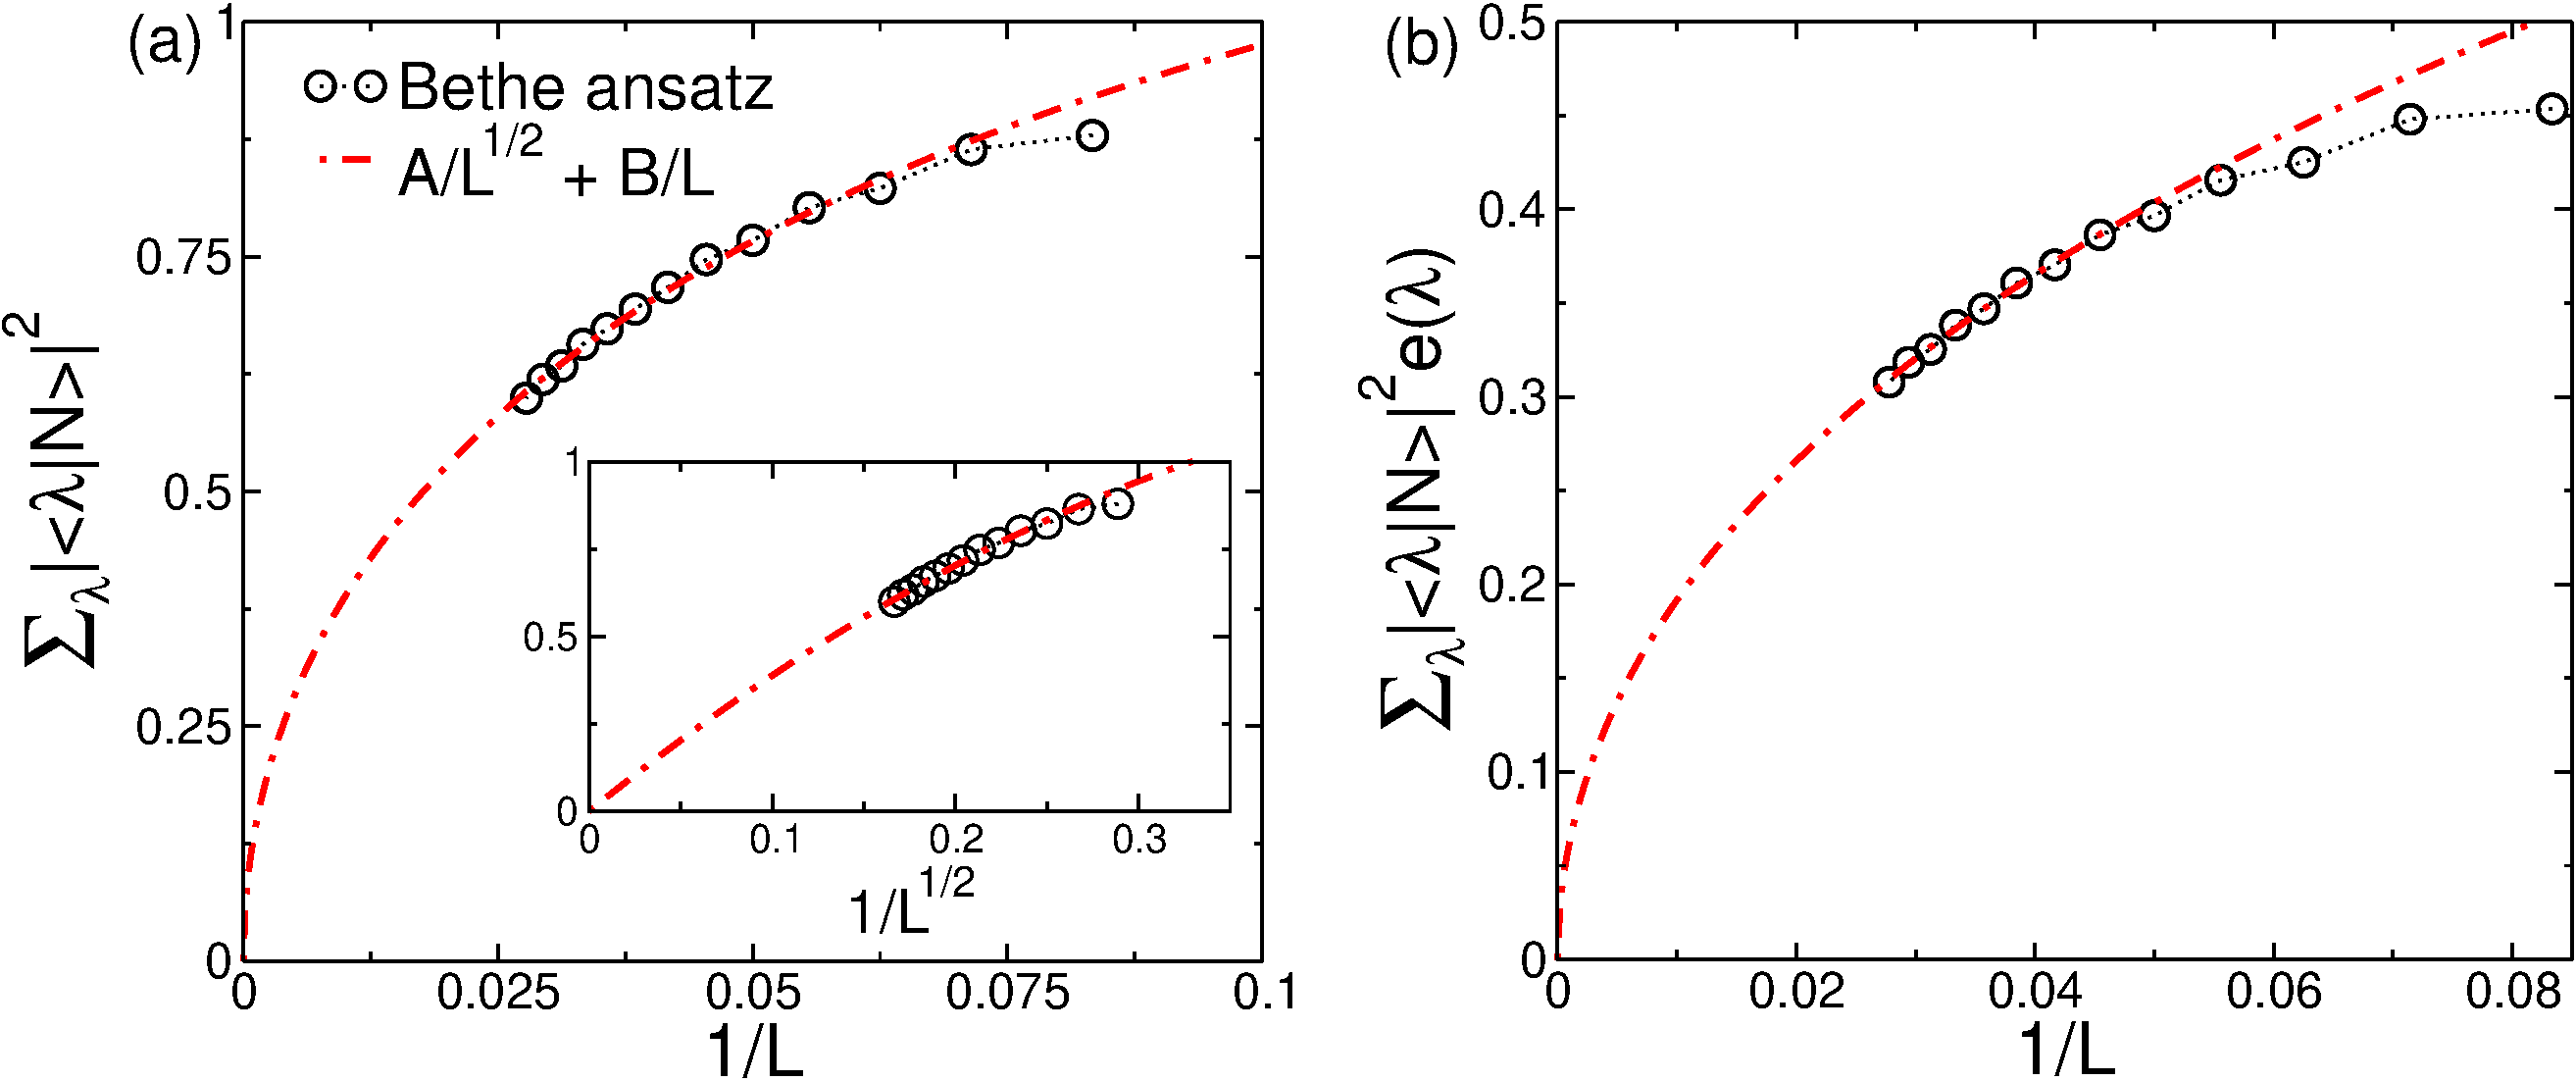
\includegraphics[width=.9\textwidth]{./draft_figs/Neel}
\end{center}
\caption{Overlap sum rules for the N\'eel state $|N\rangle$: The role of 
 the zero-momentum strings. (a) The overlap sum rule $\sum_{\lambda}|
 \langle\lambda|N\rangle|^2=1$. Here $|\lambda\rangle$ are the eigenstates  
 of the $XXX$ chain. The $x$-axis shows the inverse chain length $1/L$. 
 The circles are Bethe ansatz results for chains up to $L=38$. The data  
 are obtained by  a full scanning of the chain Hilbert space. Eigenstates  
 corresponding to zero-momentum strings are excluded. The dotted line is 
 the expected result at any $L$. The data are compatible with a vanishing 
 behavior in the thermodynamic limit. The dash-dotted line is a fit to 
 $A/L^{1/2}+B/L$, with $A,B$ fitting parameters. Inset: The same data as 
 in the main Figure now plotted versus $1/L^{1/2}$. (b) 
 The same as in (a) for the energy sum rule $\sum_{\lambda}|\langle
 \lambda|N\rangle|^2Q_2(\lambda)=Q_2^{(0)}$, with $Q_2(\lambda)$ the 
 energy of the eigenstate $|\lambda\rangle$ and $Q_2^{(0)}/L=-1/2$ the 
 N\'eel state energy density (dotted line in the Figure). 
}
\label{fig1:neel-sr}
\end{figure}
%##################################################################

Here we illustrate the effect of the zero-momentum strings eigenstates on the 
N\'eel overlap sum rules. We focus on the ``trivial'' sum rule, i.e., the 
normalization of the N\'eel state  
%
\begin{equation}
\label{sr-trivial}
\langle N|N\rangle=\sum\limits_{\lambda}|\langle\lambda|N\rangle|^2=1. 
\end{equation}
%
We also consider the N\'eel expectation value of the local conserved charge 
$Q_n$ of the $XXX$ chain (see subsection~\ref{sec:1.5}). These provide the 
additional sum rules
%
\begin{equation}
\label{sr-charge}
Q_n^{(0)}=\langle N|Q_n|N\rangle=\sum\limits_{\lambda}|\langle\lambda|N\rangle|^2
Q_{n}(\lambda)\quad\textrm{with}\quad n\in\mathbb{N}, 
\end{equation}
%
where $Q_n(\lambda)$ are the charges eigenvalues over the generic Bethe state 
$|\lambda\rangle$ (cf.~\eref{qngnk} and~\eref{gnk}). In both~\eref{sr-trivial} 
and~\eref{sr-charge} the sums are restricted to the eigenstates with no zero-momentum 
strings. In~\eref{sr-charge} $Q_n^{(0)}$ is the expectation value of $Q_n$ over the 
initial N\'eel state. $Q_n^{(0)}$ have been calculated in Ref.~\cite{fagotti-2013} 
for any $n$. Due to the locality of $Q_n$, the translational invariance of the initial 
state, and the periodic boundary conditions, the density $Q_n^{(0)}/L$ does 
not depend on the chain size. Note also that the N\'eel state, $Q_n^{(0)}$ can be 
calculated directly in the thermodynamic limit using~\eref{q0-th} and the root 
distributions $\pmb{\rho}^*$ (cf.~\eref{rho1-sp}-\eref{rho3-sp}). 

The sum rules~\eref{sr-trivial} and~\eref{sr-charge} (for $n=2$, i.e., the energy 
sum rule), are shown in Figure~\ref{fig1:neel-sr} (a) and (b), respectively. 
Note that $Q^{(0)}_2/L=-1/2$ in~\eref{sr-charge} (horizonthal dotted line). 
The circles in Figure~\ref{fig1:neel-sr} (a) are the Bethe ansatz results excluding 
the zero momentum strings. The data are the same as in Figure~\ref{fig0:neel-ov}. 
The sum rules are plotted against the inverse chain length $1/L$, for $L\le 38$. 

Clearly, both the sum rules are violated, due to the exclusion of the to zero-momentum 
strings. Moreover, in both Figure~\ref{fig1:neel-sr} (a) and (b) the data suggest a 
vanishing behavior upon increasing $L$. The dash-dotted lines are fits to  $A/L^{1/2}
+B/L$, with $A,B$ fitting parameters. Interestingly, the behavior as $\propto 
L^{-1/2}$ of the sum rules reflects that of the fraction of non-zero momentum string 
eigenstates $\widetilde Z_{Neel}/Z_{Neel}$. Specifically, from~\eref{zneel1} and~\eref{ztilde} 
it is straightforward to derive that for $L\to\infty$
%
\begin{equation}
\label{beh}
\frac{\widetilde Z_{Neel}}{Z_{Neel}}\propto\frac{4}{\sqrt{\pi L}}. 
\end{equation}
% 


%##################################################################
\begin{figure}[t]
\begin{center}
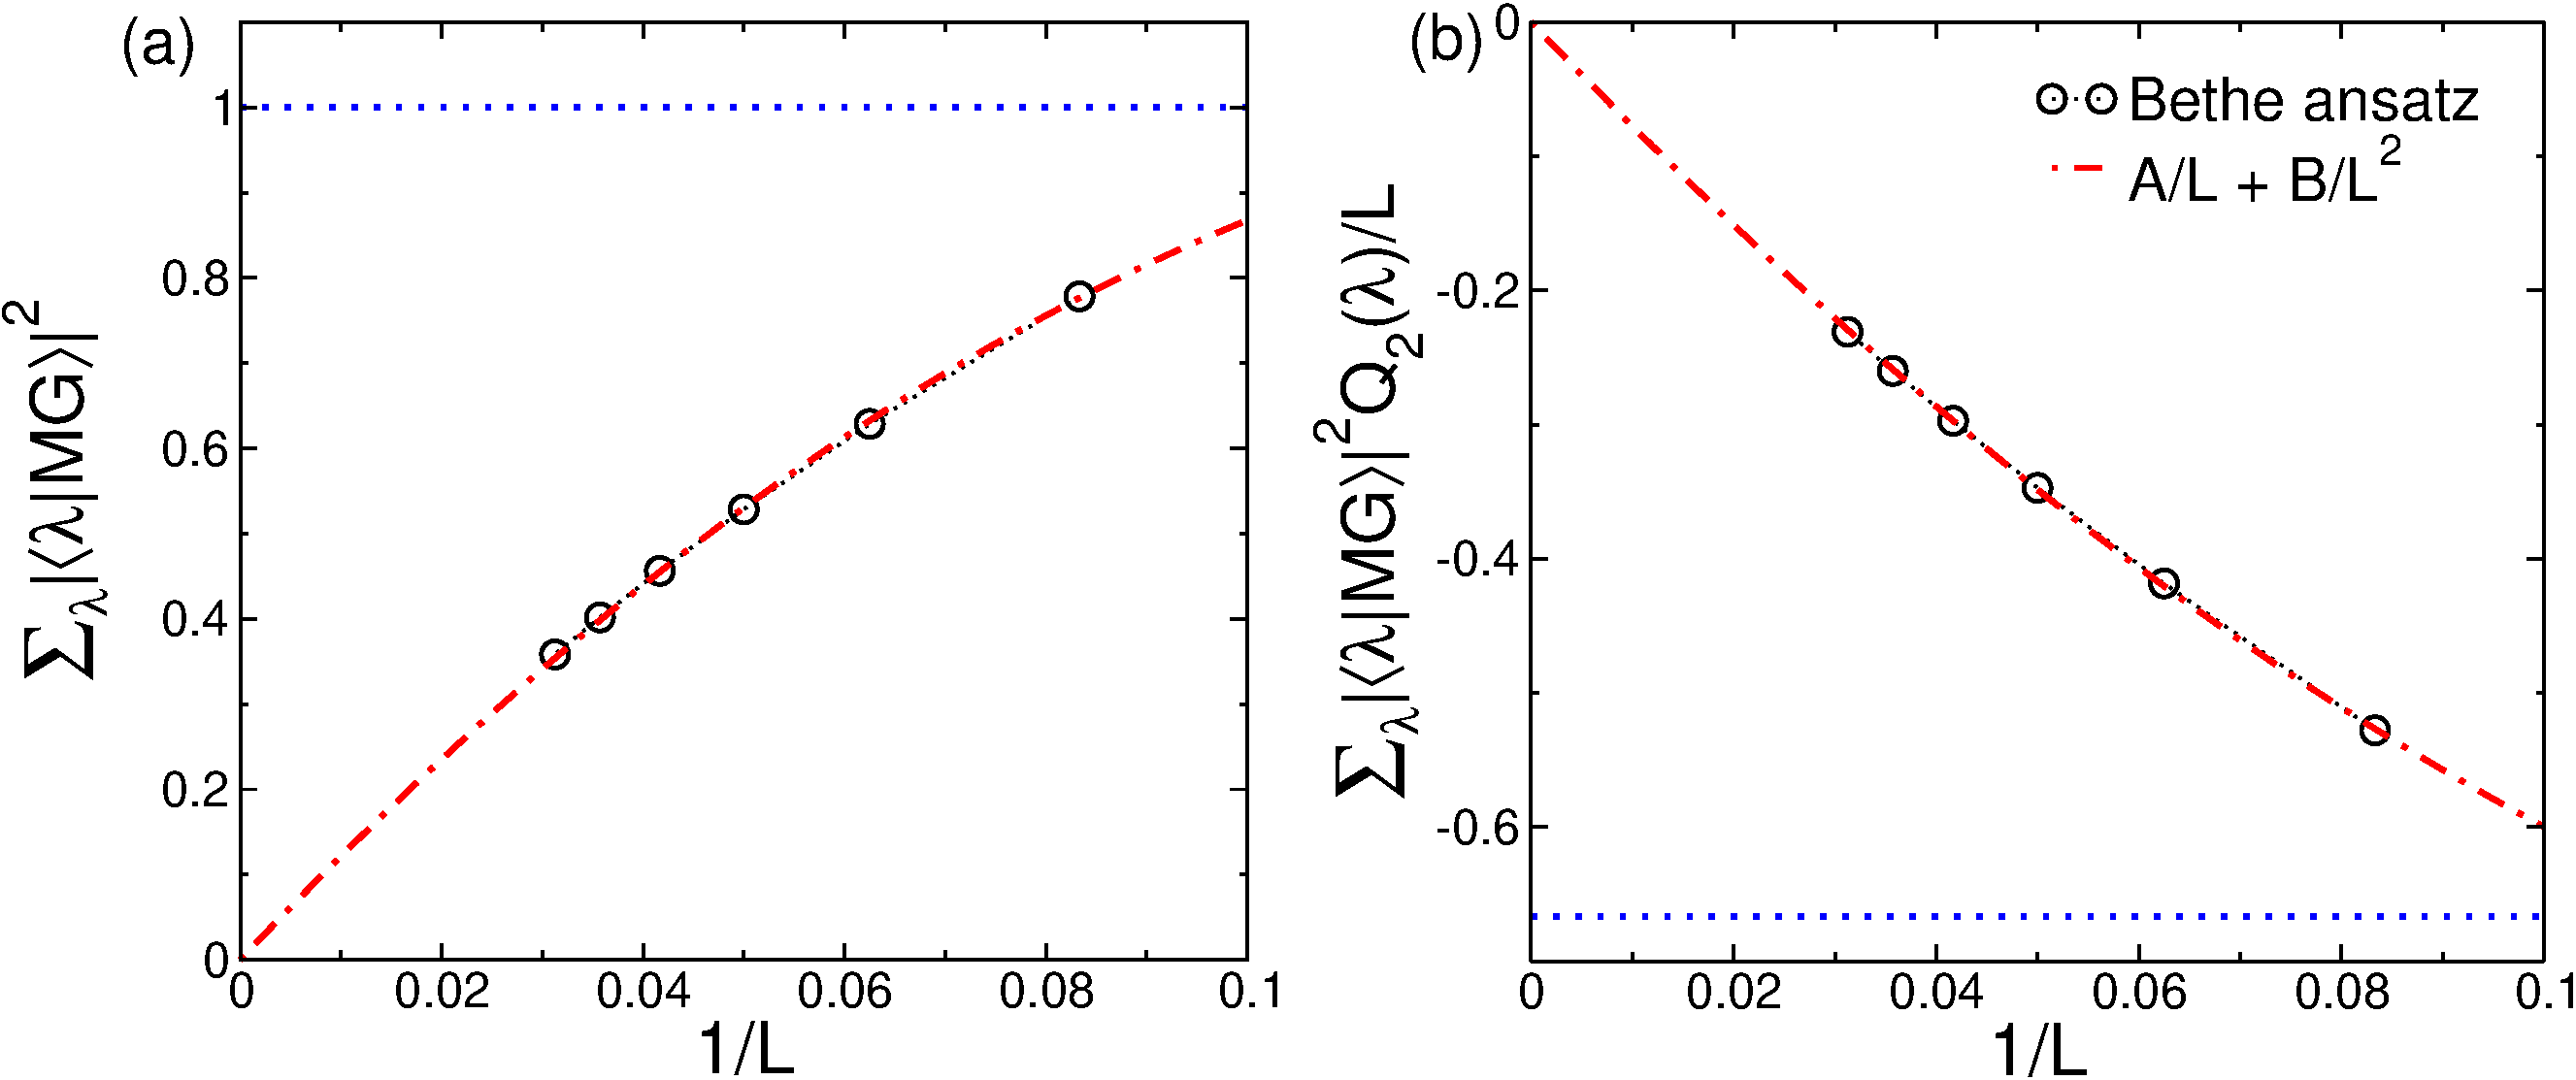
\includegraphics[width=.9\textwidth]{./draft_figs/Dimer}
\end{center}
\caption{Overlap sum rules for the Majumdar-Ghosh state $|MG\rangle$: 
 The role of the zero-momentum strings. (a) The sum rule $\sum_{\lambda}|
 \langle\lambda|MG\rangle|^2=1$, with $|\lambda\rangle$ the eigenstates   
 of the $XXX$ chain. The $x$-axis plots the inverse chain length $1/L$. 
 The circles are Bethe ansatz results for chains up to $L=32$. The results 
 are obtained by a full scanning of the chain Hilbert space. Eigenstates 
 corresponding to zero-momentum strings are excluded. The dash-dotted line 
 is a fit to $A/L+B/L^2$, with $A,B$ fitting parameters. (b) The same as 
 in (a) for the energy sum rule $\sum_{\lambda}|\langle\lambda|MG\rangle
 |^2Q_2(\lambda)=Q_2^{(0)}$, with $Q_2(\lambda)$  the energy of $|\lambda
 \rangle$ and $Q_2^{(0)}/L=-2/3$ the Majumdar-Ghosh energy density (dotted 
 line in the Figure). 
}
\label{fig2:dimer-sr}
\end{figure}
%##################################################################

It is interesting to observe that the large $L$ behavior as $L^{-1/2}$  of the sum 
rules is not generic, meaning that it depends on the pre-quench initial state $|\Psi_0
\rangle$. This is illustrated in Figure~\ref{fig2:dimer-sr}, focusing on the 
Majumdar-Ghosh (MG) state. As for the N\'eel state, only parity-invariant eigenstates 
can have non-zero Majumdar-Ghosh overlap. Their total number $Z_{MG}$ (cf.~\eref{p-inv-mg}) 
is given as 
%
\begin{equation}
\label{mg1}
Z_{MG}=B\Big(\frac{L}{2}-1,\frac{L}{4}-1\Big)+B\Big(\frac{L}{2}-1,
\frac{L}{4}-1\Big). 
\end{equation}
%
As for~\eref{zneel1}, $Z_{MG}$ is only un upper bound for the number of Bethe states with 
non-zero Majumdar-Ghosh overlaps. Note also that at any size $L$ one has $Z_{MG}<Z_{Neel}$. 
This is due to the Majumdar-Ghosh state being invariant under $SU(2)$ rotations, since it 
contains only spin singlets. In constrast with the N\'eel state, this implies that the 
Majumdar-Ghosh stat has non-zero overlap only with the $S^z_T=0$ sector of the $XXX$ chain 
spectrum. After restricting to the situation with no zero-momentum strings, the total number 
of parity-invariant eigenstates $\widetilde Z_{MG}$ in the sector with $S_T^z=0$ is now 
(cf.~\eref{mg-fi})
%
\begin{equation}
\label{mg2}
\widetilde Z_{MG}=B\Big(\frac{L}{2},\frac{L}{4}\Big)-B\Big(\frac{L}{2},
\frac{L}{4}-1\Big). 
\end{equation}
%
Panels (a) and (b) in Figure~\ref{fig2:dimer-sr} plot the sum rules~\eref{sr-trivial} 
and~\eref{sr-charge} for the Majumdar-Ghosh state. The data are obtained using the 
analytic results for the overlaps in subsection~\ref{sec:2.3}. The expected value for 
the energy density sum rule is $Q_2^{(0)}=-2/3$ (horizonthal dotted line in 
Figure~\ref{fig2:dimer-sr} (b)). Similar to Figure~\ref{fig1:neel-sr}, due to the exclusion 
of the zero-momentum strings, the sum rules are violated, exhibiting vanishing behavior in 
the thermodynamic limit. However, in contrast with the N\'eel case, one has the behavior 
as $1/L$, as confirmed by the fits (dash-dotted lines in Figure~\ref{fig2:dimer-sr}). 
Similar to the N\'eel case, the vanishing of the sum rules in the thermodynamic limit 
reflects the behavior of $\widetilde Z_{MG}/Z_{MG}$ as (see~\eref{mg1} and~\eref{mg2})
%
\begin{equation}
\frac{\widetilde Z_{MG}}{Z_{MG}}=\frac{4}{4+L}. 
\end{equation}
%


%%%%%%%%%%%%%%%%%%%%%%%%%%%%%%%%%%%%%%%%%%%%%%%%%%%%%%%%%%%%%%%%%%%%%%%%%%%
\section{Monte Carlo implementation of the quench action approach}
\label{sec6:mcqa}

In this section, by generalizing the results in~\cite{alba-2015}, we present 
a Monte Carlo implementation of the quench action approach for the N\'eel quench in 
the $XXX$ chain. The key idea is to sample the eigenstates of the finite-size $XXX$ 
chain with the quench action probability distribution, given in~\eref{qa-d-ensemble}. 
Importantly, we consider a truncated Hilbert space, restricting ourselves to the 
eigenstates corresponding to solutions of the BGT equations with no zero-momentum 
strings. Our main physical result is that, despite this restriction, the remaining 
eigenstates contain enough information to correctly reproduce the post-quench 
thermodynamic behavior of the $XXX$ chain. 

In subsection~\ref{sec:6.1} we detail the Monte Carlo algorithm. In 
subsection~\ref{sec:6.2} we numerically demonstrate that after the Monte Carlo 
``resampling'' the N\'eel sum rules~\eref{sr-charge} are restored, in the 
thermodynamic limit. The Hilbert space truncation is reflected only in 
$\propto 1/L$ finite-size corrections to the sum rules. In the Bethe ansatz 
language the eigenstates sampled by the Monte Carlo become equivalent to the 
quench action representative state in the thermodynamic limit. Here this is 
explicitly demonstrated by numerically extracting the quench action root 
distributions $\pmb{\rho}^*$ (cf.~\eref{rho1-sp}-\eref{rho3-sp}). The 
numerical results are found in remarkable agreement with the quench action. 



%%%%%%%%%%%%%%%%%%%%%%%%%%%%%%%%%%%%%%%%%%%%%%%%%%%%%%%%%%%%%%%%%%%%%%%%%%%
\subsection{The quench action Monte Carlo algorithm}
\label{sec:6.1}


The Monte Carlo procedure starts with a randomly selected parity-invariant eigenstate 
(Bethe state) of the $XXX$ chain, in the sector with zero magnetization, i.e., $M=L/2$ 
particles. As the N\'eel state is not invariant under $SU(2)$ rotations, in order to 
characterize the Bethe states one has to specify the number $N_{\infty}$ of infinite 
rapidities (see~\ref{sec:1.2}). The number of remaining particles corresponding to finite 
BGT rapidities $M'$ is $M'=L/2-N_\infty$. The Bethe state is identified by a parity-invariant 
BGT quantum number configuration that we denote as ${\mathcal C}$. Due to the parity-invariance 
and the zero-momentum strings being excluded, ${\mathcal C}$ is identified by the 
number $m'$ of parity-invariant quantum numbers $\{\pm I_j\}_{j=1}^{m'}$ (equivalently, 
root pairs $\{\pm\lambda_j\}_{j=1}^{m'}$). The string 
content associated with the state is denoted as $\widetilde{\mathcal S}=\{\tilde s_1,
\dots,\tilde s_{m'}\}$, where $\tilde s_n$ is the number of pairs of $n$-strings. The 
Monte Carlo procedure generates a new parity-invariant eigenstate of the $XXX$ chain, 
and it consists of four steps: 
%
\begin{enumerate}
\item[\circled{1}] Choose a new number of finite-momentum particles $M''$ and of 
parity-invariant rapidity pairs $m''\equiv M''/2$ with 
probability ${\mathcal P}(M'')$ as 
%
\begin{equation}
\label{PM}
{\mathcal P}(M'')=\frac{\widetilde Z'_{Neel}(L,M'')}
{\widetilde{Z}_{Neel}(L)}, 
\end{equation}
%
where $\widetilde Z_{Neel}(L)$ is defined in~\eref{ztilde}, and $\widetilde 
Z'_{Neel}$ is the number of parity-invariant eigenstates with no zero-momentum 
strings in the sector with fixed particle number $M''$  (cf.~\eref{neel-fi} for 
the precise expression). 
\item[\circled{2}] Choose a new string content $\widetilde{\mathcal S}'\equiv
\{\tilde s_1',\dots,\tilde s'_{m''}\}$ with probability ${\mathcal P}'(M'',
\widetilde{\mathcal S}')$
%
\begin{equation}
\label{PS}
{\mathcal P}'(M'',\widetilde{\mathcal S}')=\frac{1}{\widetilde Z'_{Neel}
(L,M'')}\prod_{n=1}^{m''}B\Big(\frac{L}{2}-\sum\limits_{l=1}^{
m''}t_{nl}\tilde s'_l,\tilde s'_n\Big), 
\end{equation}
%
where the matrix $t_{nl}$ is defined in~\eref{bt-qn-bound}.
\item[\circled{3}] Generate a new parity-invariant quantum number configuration 
${\mathcal C}'$ compatible with the $\widetilde {\mathcal  S}'$ obtained in step 
$\circled{2}$. Solve the corresponding BGT equations~\eref{bgt-eq}, finding the 
rapidities $\{\pm\lambda'_j\}_{j=1}^{m''}$ of the new parity-invariant eigenstate. 
\item[\circled{4}] Calculate the N\'eel overlap $\langle\{\pm\lambda'_j\}_{j=1}^{m''}
|N\rangle$ for the new eigenstate,  using~\eref{neel-ov}~\eref{red-G+}~\eref{red-G-} 
and~\eref{neel-k}. Accept the new eigenstate with the quench action Metropolis 
probability 
%
\begin{equation}
\label{metropolis}
{\mathcal P}''_{\lambda\to\lambda'}=\textrm{Min}\Big\{1,\exp\Big(-
2\Re({\mathcal E}'-{\mathcal E})\Big)\Big\}, 
\end{equation}
%
where ${\mathcal E}'\equiv-\log\langle\{\pm\lambda'_j\}_{j=1}^{m''}
|N\rangle$, ${\mathcal E}\equiv-\log\langle\{\pm\lambda_j\}_{j=1}^{m''}
|N\rangle$, and $\Re$ denoting the real part. 
\end{enumerate}
%
Note that while the steps $1$-$3$ account for the string content and particle 
number probabilities of the parity-invariant states, step $4$ assigns to the 
different eigenstates the correct quench action probability. 

For a generic observable ${\mathcal O}$, its quench action $\langle{\mathcal O}
\rangle$ is obtained from the Monte Carlo simulation as the arithmetic average 
of the eigenstates expectation values $\langle\lambda|{\mathcal O}|\lambda\rangle$, 
with $|\lambda\rangle$ the eigenstates sampled by the Monte Carlo, as 
%
\begin{equation}
\label{qamc-obs}
\langle{\mathcal O}\rangle=\frac{1}{N_{mcs}}\sum\limits_{\lambda}\langle\lambda|
{\mathcal O}|\lambda\rangle. 
\end{equation}
%
Here $N_{mcs}$ is the total number of Monte Carlo steps. Note that, as usual in 
Monte Carlo, some initial steps have to be neglected to ensure equilibration. 
Note that~\eref{qamc-obs} can be used for any observable ${\mathcal O}$ for 
which the the Bethe state expectation value $\langle\lambda|{\mathcal O}|\lambda
\rangle$ (form factor) is known. 


%%%%%%%%%%%%%%%%%%%%%%%%%%%%%%%%%%%%%%%%%%%%%%%%%%%%%%%%%%%%%%%%%%%%%%%%%%%
\subsection{The N\'eel overlap sum rules: Monte Carlo results}
\label{sec:6.2}

%##################################################################
\begin{figure}[t]
\begin{center}
\includegraphics[width=.9\textwidth]{./draft_figs/QAMC_Obs_Neel}
\end{center}
\caption{The overlap sum rules for the N\'eel state $|N\rangle$ in the 
 Heisenberg spin chain: Numerical results obtained by the Monte Carlo 
 sampling of the chain Hilbert space. In all panels the $x$ axis shows 
 the inverse chain length $1/L$ (a) The energy sum rule $\sum_\lambda|
 \langle N|\lambda\rangle|^2Q_2(\lambda)/L=Q^{(0)}_2$, with $|\lambda
 \rangle$ the generic eigenstate of the $XXX$ chain, $Q_2(\lambda)/L$ 
 the associated energy density, and $Q_2^{(0)}=-1/2$ the N\'eel energy 
 density. The symbols are Monte Carlo data. The dash-dotted line is the 
 expected result $Q_2^{(0)}$. The dashed line is a fit to the behavior 
 $-1/2+A/L+B/L^2$, with $A,B$ fitting parameters. (b) The N\'eel sum rule 
 for the energy fluctuations $\sigma^2(Q_2)$ (cf.~\eref{sigma-sr} for 
 the definition). The horizontal line is the expected result $1/4$. 
 (c)(d) Same as in (a)(b) for the charge $Q_4$ and its fluctuations. 
}
\label{fig3:neel-qamc-sr}
\end{figure}
%##################################################################


The validity of the Monte Carlo approach outlined in~\ref{sec:6.2} is demonstrated 
in Figure~\ref{fig3:neel-qamc-sr} (a)-(d). The Figure focuses on the N\'eel overlap 
sum rules for the conserved charges densities $Q_2/L$ and $Q_4/L$ (cf. 
subsection~\ref{sec:1.5} for the definition of the charges, and~\eref{sr-charge} 
for the associated sum rules). Here we also consider the corresponding fluctuations 
$\sigma^2(Q_n)$, which are defined as 
%
\begin{equation}
\label{sigma-sr}
\fl\quad\sigma^2(Q_n)\equiv\langle N|Q^2_n|N\rangle-\langle N|Q_n|N\rangle^2=
\sum\limits_{\lambda}|\langle N|\lambda\rangle|^2Q^2_n(\lambda)-\Big(\sum_\lambda|
\langle N|\lambda\rangle|^2Q_n(\lambda)\Big)^2.
\end{equation}
%
Note that in both~\eref{sr-charge} and~\eref{sigma-sr} the sum is now over the 
eigenstates $|\lambda\rangle$ sampled by the Monte Carlo. 
Panel (a) and (b) in Figure~\ref{fig3:neel-qamc-sr} plot the sum rules for 
the energy density $Q_2/L$, and its density of fluctutations $\sigma^2(Q_2)/L$. 
It is straightforward to derive that $\sigma(Q_2)/L=1/4$, which is shown as dash-dotted 
line in Figure~\ref{fig3:neel-qamc-sr} (b). 
The circles in the Figure are Monte Carlo data for the Heisenberg chain with $L\le 56$ 
sites. The data correspond to Monte Carlo simulations with $N_{mcs}\sim 10^7$ Monte 
Carlo steps (mcs). In all panels the $x$-axis shows the inverse chain length $1/L$. 

Clearly, the Monte Carlo data suggest that in the thermodynamic limit the N\'eel 
overlap sum rules~\eref{sr-charge} are restored, while violations are present for 
finite chains. This numerically confirms that the truncation of the Hilbert space, 
i.e., removing the zero-momentum strings, gives rise only to scaling corrections, 
while the thermodynamic behavior after the quench is correctly reproduced. 
Note that the data in panel (a) are suggestive  of the behavior $\propto 1/L$ for 
the scaling corrections, as confirmed by the fit to $-1/2+A/L+b/L^2$ (dashed line in the Figure), 
with $A,B$ fitting parameters. The same behavior should be expected for the energy 
fluctuations $\sigma^2(Q_2)$ (panel (b) in the Figure), although the asymptotic  
behvior sets in for $L\gg 56$. 


Similarly, panels (c) and (d) in Figure~\ref{fig3:neel-qamc-sr} plot the charge 
density $Q_4/L$ and its fluctuations $\sigma^2(Q_4)/L$. While for $Q_4/L$ the Monte 
Carlo data for $L=48$ are already compatible with the expected result $Q_4/L=1/4$ 
in the thermodynamic limit, $\sigma^2(Q_4)$ exhibits large scaling corrections. 
This could be attributed to fact that the support of $Q_n$, i.e., the number of 
sites where the operator acts non trivially, increases linearly with $n$ 
(see~\cite{grabowski-1995} for the precise expression). 

%%%%%%%%%%%%%%%%%%%%%%%%%%%%%%%%%%%%%%%%%%%%%%%%%%%%%%%%%%%%%%%%%%%%%%%%%%%
\subsection{Extracting the quench action root distributions}
\label{sec:6.3}

%##################################################################
\begin{figure}[t]
\begin{center}
\includegraphics[width=.95\textwidth]{./draft_figs/Neel_rho}
\end{center}
\caption{ The quench action root distributions $\rho^*_1(\lambda)$ and 
 $\rho^*_2(\lambda)$ for the $1$-strings and $2$-strings, respectively: Monte 
 Carlos results. (a) The histograms of the $1$-string Bethe-Gaudin-Takahashi 
 (BGT) roots $\lambda$ sampled in the Monte Carlo. The data are for a chain 
 with $L=56$ sites and a Monte Carlo history with $N_{mcs}\sim 10^7$ Monte 
 Carlo steps. The $y$-axis is divided by a factor $10^6$ for convenience. 
 The width of the histogram bin is $\Delta\lambda\sim 0.07$. (c) The same as 
 in (a) for the $2$-string roots. (b) The $1$-string root distribution 
 $\rho^*_1(\lambda)$ plotted versus $\lambda$ for two chains with $L=48$ 
 and $L=56$ (diamond and circles, respectively). The full line 
 is the quench action analytic result in the thermodynamic limit. (d) 
 The same as in (b) for the $2$-string root distribution $\rho^*_2(\lambda)$. 
 In both (b) and (d) the oscillations are finite-size effects, whereas 
 the error bars are the statistical Monte Carlo errors. 
}
\label{fig4:neel-rho}
\end{figure}
%##################################################################

The BGT root distributions corresponding to the quench action steady state 
(cf.~\eref{rho1-sp}-\eref{rho3-sp}) $\pmb{\rho^*}=\{\rho^*_n(\lambda)\}_{n=
1}^{\infty}$ can be extracted from the Monte Carlo simulation,  similar to 
what has been done in Ref.~\cite{alba-2015} for the Generalized Gibbs Ensemble 
(GGE) representative state. The idea is that for the local observables considered 
here, in each eigenstate expectation value $\langle\lambda|{\mathcal O}|\lambda
\rangle$ in~\eref{qamc-obs} one can isolate the contribution of the different 
string sectors as 
%
\begin{equation}
\langle\lambda|{\mathcal O}|\lambda\rangle=\sum\limits_{n,\gamma}{\mathcal O}_n
(\lambda_{n;\gamma}). 
\end{equation}
%
Here ${\mathcal O}_n$ is the contribution of the BGT $n$-strings to the expectation 
value of ${\mathcal O}$, and $\pm\lambda_{n;\gamma}$, with $\gamma$ labeling the 
different $n$-strings, are the solutions of the BGT equations~\eref{bgt-eq} 
identifying the Bethe state $|\lambda\rangle$. By comparing~\eref{qamc-obs} 
and~\eref{obs-th} one obtains that in the limit $L,N_{mcs}\to\infty$ 
%
\begin{equation}
\quad\fl\lim_{N_{mcs}\to\infty}\,\frac{1}{N_{mcs}}\sum\limits_{\lambda_{n;\gamma}}
{\mathcal O}_n(\lambda_{n;\gamma})\,\stackrel{L\to\infty}{\overrightarrow{\hspace{40pt}}}
\,\langle\pmb{\rho^*}|{\mathcal O}|\pmb{\rho^*}\rangle\equiv\sum_n\int_{-\infty}^{+\infty}d
\lambda\rho^*_{n}(\lambda){\mathcal O}_n(\lambda). 
\end{equation}
%
This suggests that the histogram of the $n$-strings BGT roots sampled in the Monte 
Carlo converges in the thermdynamic limit to the saddle point root distribution 
$\rho^*_n(\lambda)$. 

This is demonstrated numerically in Figure~\ref{fig4:neel-rho} considering $\rho^*_1(\lambda)$ 
(panels (a)(b)) and $\rho^*_2(\lambda)$ (panel (c)(d)). The histograms correspond to Monte 
Carlo data for $L=48$ and $L=56$ sites. Panel (a) and (c) show the  histograms of the 
$1$-string and $2$-string BGT roots sampled in the Monte Carlo. The $y$-axis is rescaled 
by a factor $10^6$ for convenience. The width of the histogram bins $\Delta\lambda$ is 
$\Delta\lambda\approx0.02$ and $\Delta\lambda\approx0.001$ for $\rho_1(\lambda)$ and 
$\rho_2(\lambda)$, respectively. The histogram fluctuations are due both to the finite 
statistics (finite $N_{mcs}$) and to the finite size of the chain. 

The extracted quench-action root distributions $\rho^*_1(\lambda)$ and $\rho^*(\lambda)$ 
are shown in panels (b) and (d). The data are the same as in panel (a)(c). The normalization 
of the distributions is chosen such as to match the analytical results from~\eref{rho1-sp} 
and~\eref{rho2-sp}, i.e., $\int d\lambda\rho^*_1(\lambda)\approx0.31$ and $\int d\lambda
\rho^*_2(\lambda)\approx0.015$. The Monte Carlo error bars shown in the Figure are obtained 
with a standard jackknife analysis~\cite{quenouille-1949,wolff-2004}. 
The continuous lines are the expected analytic results in the thermodynamic limit 
(cf.~\eref{rho1-sp}~\eref{rho2-sp}). 

Clearly, the Monte Carlo data are in excellent agreement with~\eref{rho1-sp} in the whole 
range $-2\le\lambda\le2$ considered. For $\rho^*_1(\lambda)$ the statistical error bars 
are smaller than the symbol size. The oscillating corrections around $|\lambda|\sim0.5$ 
are lattice effects, which decrease with incresing the chain size 
(see the data for $L=48$ in the Figure). Much larger finite-size effects are observed for 
$\rho^*_2(\lambda)$ (panel (d) in the Figure). Specifically, the corrections are larger on 
the tails of the root distribution. Moreover, the Monte Carlo error bars are clearly 
larger than for $\rho_1^*(\lambda)$. This is due to the fact that since $\int d\lambda
\rho^*_2(\lambda)/\sum_n\int d\lambda\rho_n^*(\lambda)\approx 0.04$, the Monte Carlo 
statistics available for estimating $\rho_2^*(\lambda)$ is effectively reduced as 
compared to $\rho_1^*(\lambda)$. Finally, we numerically checked that finite-size 
corrections and Monte Carlo error bars are even larger for the $3$-strings root 
distribution $\rho^*_3(\lambda)$, which makes its numerical determination more 
tricky. 

%%%%%%%%%%%%%%%%%%%%%%%%%%%%%%%%%%%%%%%%%%%%%%%%%%%%%%%%%%%%%%%%%%%%%%%%%%%
\section{Conclusions}
\label{conclusions}

We presented a Monte Carlo implementation of the quench action method for integrable 
spin chains. We focused on the spin-$1/2$ isotropic Heisenberg ($XXX$) chain, considering  
the quench from the zero-momentum N\'eel state. The method is inspired by the Monte Carlo 
approach developed in Ref.~\cite{alba-2015} to simulate the Generalized Gibbs Ensemble 
(GGE) in integrable models. The key idea is the Monte Carlo sampling of the chain Hilbert 
space with the quench action probability distribution given in~\eref{qa-prob}. 

The approach relies on the knowledge of the overlaps between the pre-quench N\'eel 
state and the $XXX$ chain  eigenstates, which have been obtained recently~\cite{
pozsgay-2014,brockmann-2014,brockmann-2014a,brockmann-2014b,brockmann-2014c,piroli-2014}. 
The method is based on the detailed knowledge of the Hilbert space structure of the model 
provided by the Bethe ansatz formalism, in particular, on the so-called string hypothesis, 
and on the Bethe-Gaudin-Takahashi (BGT) equations. Although the approach is devised for 
finite-size systems, thermodynamic quantities can be extracted using finite-size scaling. 
Importantly, we restricted ourselves to a truncated Hilbert space, which is obtained by 
excluding the chain eigenstates containing zero-momentum strings. The reason is that 
zero-momentum strings lead to singularities in the N\'eel overlap formulas, which are 
tricky to deal with in the framework of the string hypothesis. Note that it has been 
argued that the physical effects of these eigenstates should be irrelevant in the 
thermodynamic limit~\cite{brockmann-2014}. 

In order to understand the effect of the zero-momentum strings in {\it finite} chains 
we first investigated the full overlap distribution function for chains up to $L=38$ sites. 
The eigenstates having, in principle, non-zero N\'eel overlap are the so-called 
parity-invariant eigenstates. Their total number is given in terms of the chain length 
by a simple combinatorial formula that we provided. We also provided additional  
formulas for the total number of eigenstates with non-zero N\'eel overlap and no 
zero-momentum strings, in the different magnetization sectors, and for fixed eigenstate 
``string content''. We found that for any finite chain the majority of eigenstates 
contain zero-momentum strings. Specifically, the fraction of eigenstates with nonzero-momentum 
strings vanishes as $L^{-1/2}$ in the thermdodynamic limit. This is dramatically reflected 
in the N\'eel overlap sum rules for the local conserved charges of the $XXX$ chain. 
Although for any chain size their value is fixed by the N\'eel state expectation 
value, violations are observed. Moreover, the sum rules vanish as $L^{-1/2}$ in the 
thermodynamic limit. This behavior reflects the vanishing of the fraction of 
eigenstates with no zero-momentum strings, confirming that their contribution 
cannot be trivially neglected. This behavior as $L^{-1/2}$, however, is not generic, 
but it depends on the pre-quench initial state. This was demonstrated here by 
considering the quench from the Majumdar-Ghosh state. We observed that the sum 
rules vanish as $1/L$, again reflecting the vanishing as $1/L$ of the fraction of 
eigenstates with no zero-momentum strings. 

Finally, we presented a Monte Carlo implementation of the quench action method. 
We numerically demonstrated the validity of the approach focusing on the N\'eel 
overlap sum rules for the local conserved quantities of the $XXX$ chain. Although 
for finite chains violations of the sum rules are present, their effect decays 
as $1/L$ upon increasing the chain size, meaning that overlap sum rules are 
restored in the thermodynamic limit. This implies that the only effect of the 
Hilbert space truncation is to give rise to scaling corrections. Physically, 
this means that the remaining eigenstates after the Hilber space truncation 
contain enough information about the post-quench thermodynamic behavior of the 
model. Finally, following Ref.~\cite{alba-2015} we extracted from the Monte Carlo 
the quench action BGT root distributions. Although finite-size corrections are 
present, already for relatively small chains with $L=56$ sites, the first two 
BGT root distributions are in impressive agreement with the analytic (quench action) 
result in the thermodynamic limit. 

%%%%%%%%%%%%%%%%%%%%%%%%%%%%%%%%%%%%%%%%%%%%%%%%%%%%%%%%%%%%%%%%%%%%%%%%%%%
\section*{Acknowledgments}

We are very grateful to ... for discussions. V.~A. and P.~C acknowledge 
support by the ERC under Starting Grant 279391 EDEQS. 


%%%%%%%%%%%%%%%%%%%%%%%%%%%%%%%%%%%%%%%%%%%%%%%%%%%%%%%%%%%%%%%%%%%%%%%%%%%
\appendix

%%%%%%%%%%%%%%%%%%%%%%%%%%%%%%%%%%%%%%%%%%%%%%%%%%%%%%%%%%%%%%%%%%%%%%%%%%%
\section{Counting and string content of the eigenstates with nonzero N\'eel and 
Majumdar-Ghosh overlap}
\label{app-1}

Here we provide some exact combinatorial formulas for the total number of 
parity-invariant eigenstates of the $XXX$ chain having non-zero overlap with 
the N\'eel state and the Majumdar-Ghosh state. 
%We consider both the situations  
%with constrained and unconstrained string content and particle number (i.e., 
%total magnetization). 
In~\ref{app-1.1} we consider all possible parity-invariant 
eigenstates, whereas in~\ref{app-1.2} we exclude the eigenstates containing 
zero-momentum strings. Note that the result in~\ref{app-1.1} is only an upper 
bound, while the counting in~\ref{app-1.2} is exact. The strategy of the proof 
is the same as that used to count the number of solutions of the 
Bethe-Gaudin-Takahashi equations (see for instance Ref.~\cite{faddeev-1996}). 

%%%%%%%%%%%%%%%%%%%%%%%%%%%%%%%%%%%%%%%%%%%%%%%%%%%%%%%%%%%%%%%%%%%%%%%%%%%
\subsection{Allowing the zero-momentum strings}
\label{app-1.1}


Here we prove that the total number of parity-invariant eigenstates $Z_{Neel}$ 
with, in principle, non-zero N\'eel overlap for a chain of length $L$ is given 
as 
%
\begin{equation}
\label{N-count}
Z_{Neel}=2^{\frac{L}{2}-1}+\frac{1}{2}B\Big(\frac{L}{2},\frac{L}{4}\Big)+1. 
\end{equation}
%
We restrict ourselves to the situation with $L$ divisible by four. The strategy to 
prove~\eref{N-count} is to count all the possible parity-invariant BGT quantum numbers 
configurations (cf. section~\ref{sec:1.3}). Let us consider the sector with fixed number 
of particles $M$, and string content ${\mathcal S}=\{s_1,s_2,\dots,s_{M}\}$. Here $s_n$ is 
the number of $n$-strings, with the constraint $\sum_k ks_k=M$. One should stress that 
$M$ is the number of particles corresponding to {\it finite} solutions of the Bethe 
equations. The total number of particles is $L/2$, due to the fact that the N\'eel 
state has $S_T^z=0$. The remaining $L/2-M$ particles correspond to infinite solutions 
of the Bethe equations (see section~\ref{sec:1.2}). It is straightforward to check that 
total number of parity-invariant quantum number pairs ${\mathcal N}_n(L,{\mathcal S})$ 
in the $n$-string sector is given as 
%
\begin{equation}
\label{NnLS}
{\mathcal N}_n(L,{\mathcal S})=\Big\lfloor\frac{L}{2}-\frac{1}{2}
\sum_{m=1}^{M}t_{nm}s_m\Big\rfloor,
\end{equation}
%
where $t_{nm}\equiv 2\textrm{Min}(n,m)-\delta_{n,m}$. Thus, the number of parity-invariant 
eigenstates of the $XXX$ chain ${\mathcal N}(L,{\mathcal S})$ compatible with string content 
${\mathcal S}$ is obtained by choosing in all the possible ways the associated parity-invariant 
quantum number pairs as     
%
\begin{equation}
\label{NLS}
{\mathcal N}(L,{\mathcal S})=\prod_{m=1}^{M} B\left({\mathcal N}_m,\left\lfloor
\frac{s_m}{2}\right\rfloor\right).
\end{equation}
%
Here the product is because each string sector is treated independently, while the 
factor $1/2$ in $s_m/2$ is because since all quantum numbers are organized in pairs, 
only half of them have to be specified. Note that in each $n$-string sector only one 
zero momentum (i.e., zero quantum number) string is allowed, due to the fact that 
repeated solutions of the BGT equation are discarded. Moreover, from~\eref{NnLS} one has 
that $s_m$ is odd (even) only if this zero momentum string is (not) present. Finally, 
the floor function $\lfloor\cdot\rfloor$ in~\eref{NLS} reflects that the quantum number 
of zero-momentum strings is fixed. 

We now proceed to consider the string configurations with fixed particle number $0\le\ell
\le M$ and fixed number of strings $1\le q\le M/2$. Note that the maximum allowed string 
length is $M/2$ beacause of parity invariance. Note also that in determining $q$, strings 
of different length are treated equally, i.e., $q=\sum_m s_m$. For a given fixed pair 
$\ell,q$ the total number of allowed quantum number configurations by definition is given 
as 
%
\begin{equation}
\label{NLlq}
{\mathcal N}'(L,\ell,q)=\sum\limits_{\{\{s_m\}\,:\, \sum m s_m=\ell, \sum s_m=q\}}
{\mathcal N}(L,{\mathcal S}),
\end{equation}
%
where the sum is over the string content $\{s_m\}_{m=1}^M$ compatible with the constraints 
$\sum_m s_m=q$ and $\sum_m m s_m=\ell$. The strategy now is to write a recursive relation 
in both $\ell,q$ for ${\mathcal N}'(L,\ell,q)$. It is useful to consider a shifted string 
content ${\mathcal S}'$ defined as  
%
\begin{equation}
{\mathcal S}'\equiv \{s_{m+1}\}\quad\textrm{with}\, s_m\in{\mathcal S},\,\forall m.
\end{equation}
%
Using the definition of $t_{ij}$, it is straightforward to derive that  
%
\begin{equation}
t_{ij}=t_{i-1,j-1}+2,
\end{equation}
%
which implies that ${\mathcal N}_n(L,{\mathcal S})$ (see~\eref{NnLS}) satisfies the 
recursive equation 
%
\begin{equation}
\label{inter}
{\mathcal N}_n(L,{\mathcal S})={\mathcal N}_{n-1}(L-2q,{\mathcal S}'). 
\end{equation}
%
After substituting~\eref{inter} in~\eref{NLS} one obtains 
%
\begin{equation}
\label{NLSr}
{\mathcal N}(L,{\mathcal S})=B\Big({\mathcal N}_1(L,{\mathcal S}),\Big\lfloor 
\frac{s_1}{2}\Big\rfloor\Big){\mathcal N}(L-2q,{\mathcal S}'). 
\end{equation}
%
Finally, using~\eref{NLSr} in~\eref{NLlq}, one obtains a recursive relation for 
${\mathcal N}'(L,\ell,q)$ as 
%
\begin{equation}
\label{NpLlq}
{\mathcal N}'(L,\ell,q)=\sum_{s=0}^{q-1}B\Big(\frac{L}{2}-q+\Big\lfloor
\frac{s}{2}\Big\rfloor,\left\lfloor\frac{s}{2}\right\rfloor\Big){\mathcal N}'
\left(L-2q,\ell-q,q-s\right), 
\end{equation}
%
with the condition that for $\ell=q$ one has 
%
\begin{equation}
{\mathcal N}'(L,q,q)=B\Big(\Big\lfloor\frac{L-q}{2}\Big\rfloor,\Big\lfloor
\frac{q}{2} \Big\rfloor\Big).
\end{equation}
%
This is obtained by observing that if $\ell=q$ only $1$-strings are allowed 
and~\eref{NnLS} gives ${\mathcal N}_n(L,{\mathcal S})=\lfloor (L-q)/2\rfloor$. 
It is straightforward to check that for $q$ even the ansatz 
%
\begin{equation}
\label{inter1}
{\mathcal N}'(L,\ell,q)=\frac{q}{\ell}B\Big(\frac{L-\ell}{2},\frac{q}{2}\Big)
B\Big(\frac{\ell}{2},\frac{q}{2}\Big),
\end{equation}
% 
satisfies~\eref{NpLlq}. Instead, for $q$ odd the solution of~\eref{NpLlq} is 
%
\begin{equation}
\label{inter2}
{\mathcal N}'(L,\ell,q)=\frac{\ell-q+1}{\ell}B\Big(\frac{L-\ell}{2},\frac{q-1}{2}
\Big)B\Big(\frac{\ell}{2},\frac{q-1}{2}\Big).
\end{equation}
%
The number of eigenstates in the sector with $\ell$ particles having nonzero N\'eel 
overlap $Z'_{Neel}(L,\ell)$ is obtained from~\eref{inter1} and~\eref{inter2} by 
summing over all possible values of $q$ as 
%
\begin{equation}
\label{sum1}
Z'_{Neel}(L,\ell)=\sum\limits_{q=1}^\ell {\mathcal N}'(L,\ell,q).
\end{equation}
%
It is convenient to split the summation in~\eref{sum1} considering odd and even 
$q$ separately. For $q$ odd one obtains 
%
\begin{equation}
\sum\limits_{k=0}^{\ell/2-1} {\mathcal N}'(L,\ell,2k+1)=B\Big(\frac{L}{2}-1,
\frac{\ell}{2}-1\Big),
\end{equation}
%
while for $q$ even one has 
%
\begin{equation}
\sum\limits_{k=0}^{\ell/2} {\mathcal N}'(L,\ell,2k)=B\Big(\frac{L}{2}-1,
\frac{\ell}{2}\Big). 
\end{equation}
%
Putting everything together one obtains 
%
\begin{equation}
\label{N-count-p}
Z'_{Neel}(L,\ell)=B\Big(\frac{L}{2}-1,
\frac{\ell}{2}-1\Big)+B\Big(\frac{L}{2}-1,
\frac{\ell}{2}\Big). 
\end{equation}
%
The total number of eigenstates with nonzero N\'eel overlap $Z_{Neel}(L)$ 
(cf.~\eref{N-count}) is obtained from~\eref{N-count-p} by summing over the allowed 
values of $\ell=2k$ with $k=0,1,\dots,\ell/2$. Note that the sum is over $\ell$ even 
due to the parity invariance. 

Finally, it is interesting to observe that the total number $Z_{MG}$ of parity-invariant 
eigenstates having non zero overlap with the Majumdar-Ghosh state is obtained from 
Eq~\eref{N-count-p} by replacing $\ell=L/2$, to obtain 
%
\begin{equation}
\label{p-inv-mg}
Z_{MG}=B\Big(\frac{L}{2}-1,\frac{L}{4}-1\Big)+B\Big(\frac{L}{2}-1,\frac{L}{4}
\Big). 
\end{equation}
%
Physically, this is due to the fact that the Majumdar-Ghosh state is invariant under 
$SU(2)$ rotations, implying that only eigenstates with zero total spin $S=0$ can have 
non-zero overlap. 


%%%%%%%%%%%%%%%%%%%%%%%%%%%%%%%%%%%%%%%%%%%%%%%%%%%%%%%%%%%%%%%%%%%%%%%%%%%
\subsection{Excluding the zero-momentum strings}
\label{app-1.2}

Here we demonstrate that the total number of eigenstates $\widetilde Z_{Neel}(L)$ 
with nonzero N\'eel overlap, after excluding the zero-momentum strings, is given as 
%
\begin{equation}
\label{result}
\widetilde Z_{Neel}(L)=B\Big(\frac{L}{2},\frac{L}{4}\Big). 
\end{equation}
One should first observe that in a generic $M$-particle eigenstate of the $XXX$ chain, 
due to parity invariance, only $n$-strings with length $n\le M/2$ are allowed. Also, the 
string content can be written as $\widetilde{\mathcal S}\equiv\{\tilde s_1,\dots,\tilde 
s_{M/2}\}$, i.e., $\tilde s_m=0$ $\forall m>M/2$. Due to the parity invariance 
one has that $\tilde s_m$ is always even. Clearly one has $\sum_{m=1}^{M/2}m \tilde 
s_m=M$. Finally, the total number of parity-invariant quantum numbers $\widetilde{
\mathcal N}_n$ in the $n$-string sector is given as  
%
\begin{equation}
\widetilde{\mathcal N}_n(L,\widetilde{\mathcal S})=\frac{L}{2}-\frac{1}{2}
\sum_{m=1}^{M/2}t_{nm}\tilde s_m.
\end{equation}
%
The proof now proceeds as in~\ref{app-1}. One can define the total number of eigenstates 
with nonzero N\'eel overlap in the sector with fixed $\ell$ particles and $q$ different 
string types as $\widetilde{\mathcal N}'(L,\ell,q)$. It is straigtforward to show that 
$\widetilde{\mathcal N}'(L,\ell,q)$ obeys the recursive relation
%
\begin{equation}
\label{NpLlq-1}
\widetilde{\mathcal N}'(L,\ell,q)=\sum_{s=0}^{q/2-1}B\Big(\frac{L}{2}-q+s,s\Big)\widetilde
{\mathcal N}'\Big(L-2q,\frac{\ell-q}{2},\frac{q}{2}-s\Big),
\end{equation}
% 
with the constraint
%
\begin{equation}
\widetilde{\mathcal N}'(L,1,1)=\frac{L}{2}-1. 
\end{equation}
%
One can check that the solution of~\eref{NpLlq-1} is given as 
%
\begin{equation}
\widetilde{\mathcal N}'(L,\ell,q)=\frac{L-2\ell+2}{L-\ell+2}B\Big(\frac{L-\ell}{2}+1,q\Big)
B\Big(\frac{\ell}{2}-1,\frac{q}{2}-1\Big).
\end{equation}
%
After summing over the allowed values of $q=2k$ with $k=1,2,\dots,\ell/2$ one obtains 
the total number of eigenstaets with nonzero N\'eel overlap at fixed number of 
particles $\ell$ $\widetilde Z_{Neel}'(L,\ell)$ as 
%
\begin{equation}
\label{neel-fi}
\widetilde Z_{Neel}'(L,\ell)=B\Big(\frac{L}{2},\frac{\ell}{2}\Big)-
B\Big(\frac{L}{2},\frac{\ell}{2}-1\Big).
\end{equation}
%
Summing over $\ell$ one obtains~\eref{result}. Similar to~\eref{p-inv-mg} the total number 
of eigenstates $\widetilde Z_{MG}$ having non-zero overlap with the Majumdar-Ghosh state 
is obtained from~\eref{neel-fi} by replacing $\ell\to L/2$, to obtain 
%
\begin{equation}
\label{mg-fi}
\widetilde Z_{MG}=B\Big(\frac{L}{2},\frac{L}{4}\Big)-B\Big(\frac{L}{2},\frac{L}{4}-1
\Big). 
\end{equation}
%
Interestingly, using~\eref{p-inv-mg} and~\eref{mg-fi}, one obtains that the ratio 
$\widetilde Z_{MG}/Z_{MG}$ is given as 
%
\begin{equation}
\frac{\widetilde Z_{MG}}{Z_{MG}}=\frac{4}{4+L}. 
\end{equation}
%


%%%%%%%%%%%%%%%%%%%%%%%%%%%%%%%%%%%%%%%%%%%%%%%%%%%%%%%%%%%%%%%%%%%%%%%%%%%
\section{Exact N\'eel and Majumdar-Ghosh overlaps for a small Heisenberg chain} 
\label{app-L12}

In this section we provide exact diagonalization results for the overlap between the 
N\'eel state and the Majumdar-Ghosh (MG) state and all the eigenstates of the Heisenberg 
spin chain with $L=12$ sites. For the eigenstates without zero-momentum strings, we 
also provide the overlaps obtained using the string hypothesis~\eref{neel-ov}\eref{mg-ov}. 
This allows to check the validity of the string hypothesis when calculating overlaps. 
Moreover, this also provides a simple check of the counting formula~\eref{result}. 

%%%%%%%%%%%%%%%%%%%%%%%%%%%%%%%%%%%%%%%%%%%%%%%%%%%%%%%%%%%%%%%%%%%%%%%%%%%
\subsection{N\'eel overlap}
\label{app-neel}


%%%%%%%%%%%%%%%%%%%%%%%%%%%%%%%%%%%%%%%%%%
\begin{table}[h]
\scriptsize
\centering
Bethe states with nonzero N\'eel overlap ($L=12$)\\[1ex]
\begin{tabular}{rrrrrr}
\toprule
String content & $2I_n$ & $q$ & E & $|\langle\lambda|N\rangle|^2$ (exact) & $|\langle
\lambda|N\rangle|^2$ (BGT) \\[0.3em]
\toprule
6 inf & - & - & $0$ & $0.002164502165$ & $0.002164502165$\\
\midrule
\{2,0\}\, 4 inf &$1_1$ & $2$ & $-3.918985947229$ & $0.096183409244$ & $0.096183409244$\\
 &$3_1 $ & & $-3.309721467891$ & $0.011288497947$ &             $0.011288497947$\\
 &$5_1 $ & & $-2.284629676547$ & $0.004542580506$ &             $0.004542580506$\\
 &$7_1 $ & & $-1.169169973996$ & $0.002752622983$ &             $0.002752622983$\\
 &$9_1 $ & & $-0.317492934338$ & $0.002116006203$ &             $0.002116006203$\\
\midrule
\{4,0,0,0\}\, 2 inf &$1_1 3_1 $ & $4$ & $-7.070529325964$ & $0.310133033838$ &$0.310133033838$\\
  &$1_1 5_1 $ & & $-5.847128730477$ & $0.129277023687$ &           $0.129277023687$\\
  &$ 1_1 7_1$ & & $-4.570746557876$ & $0.085992436024$ &           $0.085992436024$\\
  &$ 3_1 5_1$ & & $-5.153853093221$ & $0.015256395523$ &           $0.015256395523$\\
  &$3_1 7_1 $ & & $-3.916336243695$ & $0.010091113504$ &           $0.010091113504$\\
  &$5_1 7_1 $ & & $-2.817696043731$ & $0.004059780228$ &           $0.004059780228$\\
\midrule
\{0,2,0,0\}\, 2 inf &$1_2 $ & $2$ & $-1.905667167442$ & $0.001207238321$ & $0.0012072{\color{red}45406}$\\
  &$3_2 $ & & $-1.368837200825$ & $0.002340453815$ &            $0.0023{\color{red}25724713}$\\
  &$5_2 $ & & $-0.681173793635$ & $0.001921010489$ &            $0.0019{\color{red}39001396}$\\
\midrule
\{1,0,1,0\}\, 2 inf &$0_1 0_3$ & $2$ & $-2.668031843135$ & $0.034959609810$ & -\\
\midrule
\{6,0,0,0,0,0\}\, 0 inf &$1_1 3_1 5_1$ & $6$ & $-8.387390917445$ & $0.153412152966$ & $0.153412152966$\\
\midrule
\{2,2,0,0,0,0\}\, 0 inf &$1_1 1_2$ & $4$ & $-5.401838225870$ & $0.040162686361$ & $0.04{\color{red}1042488913}$\\  
&$3_1 1_2 $ & & $-4.613929948329$ & $0.004636541934$ & $0.004{\color{red}730512604}$\\
  &$5_1 1_2 $ &  & $-3.147465758841$ & $0.001335522556$ & $0.00133{\color{red}7334035}$\\
\midrule
\{3,0,1,0,0,0\}\, 0 inf &$0_1 2_1 0_3$ & $4$ & $-6.340207488736$ & $0.052743525774$ & -\\
  &$0_1 4_1 0_3$ & & $-5.203653009936$ & $0.015022005621$ & - \\
  &$0_1 6_1 0_3$ & & $-3.788693957250$ & $0.011144489334$ & - \\
\midrule
\{1,0,0,0,1,0\}\, 0 inf &$0_1 0_5$ & $2$ & $-2.444293750583$ & $0.005887902992$ & - \\
\midrule
\{0,0,2,0,0,0\}\, 0 inf &$1_3$ & $2$ & $-1.111855930538$ & $0.001342476001$ & $0.0013{\color{red}84980817}$ \\
\midrule
\{0,1,0,1,0,0\}\, 0 inf &$0_2 0_4$ & $2$ &  $-1.560671012472$ & $0.000026982174$ & - \\
\bottomrule
\end{tabular}
\caption{All Bethe states for $L=12$ having nonzero overlap with the zero-momentum N\'eel state. 
 The first column shows the string content of the Bethe states, including the number of infinite 
 rapidities. The second and third column show $2I_n$, with $I_n$ the BGT quantum numbers 
 identifying the different states, and the number $q$ of independent strings. Due to the parity invariance, 
 only positive quantum numbers are reported. In the second 
 column only the positive BGT numbers are shown. The fourth column is the Bethe state eigenenergy. 
 Finally, the last two columns show the exact overlap with the N\'eel state and the approximate 
 result obatained using the BGT equations. In the last column Bethe states containing zero-momentum 
 strings are excluded. Deviations from the exact result (digits with different colors) are 
 attributed to the string hypothesis. 
}
\label{table:neel}
\end{table}
%%%%%%%%%%%%%%%%%%%%%%%%%%%%%%%%%%%%%%%%%%



The overlaps between all the eigenstates of the Heisenberg spin chain and the N\'eel 
state are reported in Table~\ref{table:neel}. The first column in the Table shows 
the string content ${\mathcal S}\equiv\{s_1,\dots,s_M\}$, with $M$ being the number 
of finite rapidities. The number of infinite rapidities $N_{\infty}=L/2-M$ (see 
section~\ref{sec:1.2}) is also reported. The second column shows $2I_n$, with $I_n$ 
the Bethe-Gaudin-Takahashi quantum numbers (see section~\ref{sec:1.3}) identifying 
the $XXX$ chain eigenstates. Due to the parity invariance, only the positive quantum 
numbers are reported. The total number of independent strings, i.e., $q\equiv\sum_js_j$, 
is shown in the third column. The fourth column is the eigenstates energy eigenvalue 
$E$. The last two columns show the squared N\'eel overlaps and the corresponding result 
obtained using the Bethe-Gaudin-Takahashi equations, respectively. In the last 
column only the case with no zero-momentum strings is considered. The deviations 
from the exact diagonalization results (digits with different colors) have to be 
attributed to the string hypothesis. Notice that the overlap between the N\'eel 
state and the $S_z=0$ eigenstate in the sector with maximal total spin $S=L/2$ 
(first column in Table~\ref{table:neel}), is given analytically as $2/B(L,L/2)$, 
with $B(x,y)$ the Newton binomial. 

Some results for a larger chain with $L=20$ sites are reported in 
Figure~\ref{fig1-BGT-check}.  The squared overlaps $|\langle\lambda|
N\rangle|^2$ between the N\'eel state and the $XXX$ chain eigenstates $|\lambda
\rangle$ are plotted against the eigenstate energy density $E/L
\in[-\log(2),0]$. The circles are exact diagonalization results for all 
the chain eigenstates ($382$ eigenstates), whereas the crosses denote the 
overlaps calculated using formula~\eref{neel-ov}. Note that only the 
eigenstates with no zero-momentum strings are shown ($252$ eigenstates) 
in the Figure. Panel (a) gives an overview of all the overlaps. Panels (b)-(d) 
correspond to zooming to the smaller overlap values $|\langle N|\lambda
\rangle|\lesssim 0.02$, $|\langle N|\lambda\rangle|\lesssim 0.002$, and 
$|\langle N|\lambda\rangle|\lesssim 10^{-5}$. 
Although some deviations are present, the overall agreement between the exact 
diagonalization results and the Bethe ansatz is satisfactory, confirming 
the validity of the string hypothesis for overlap calculations. 


%##################################################################
\begin{figure}[t]
\begin{center}
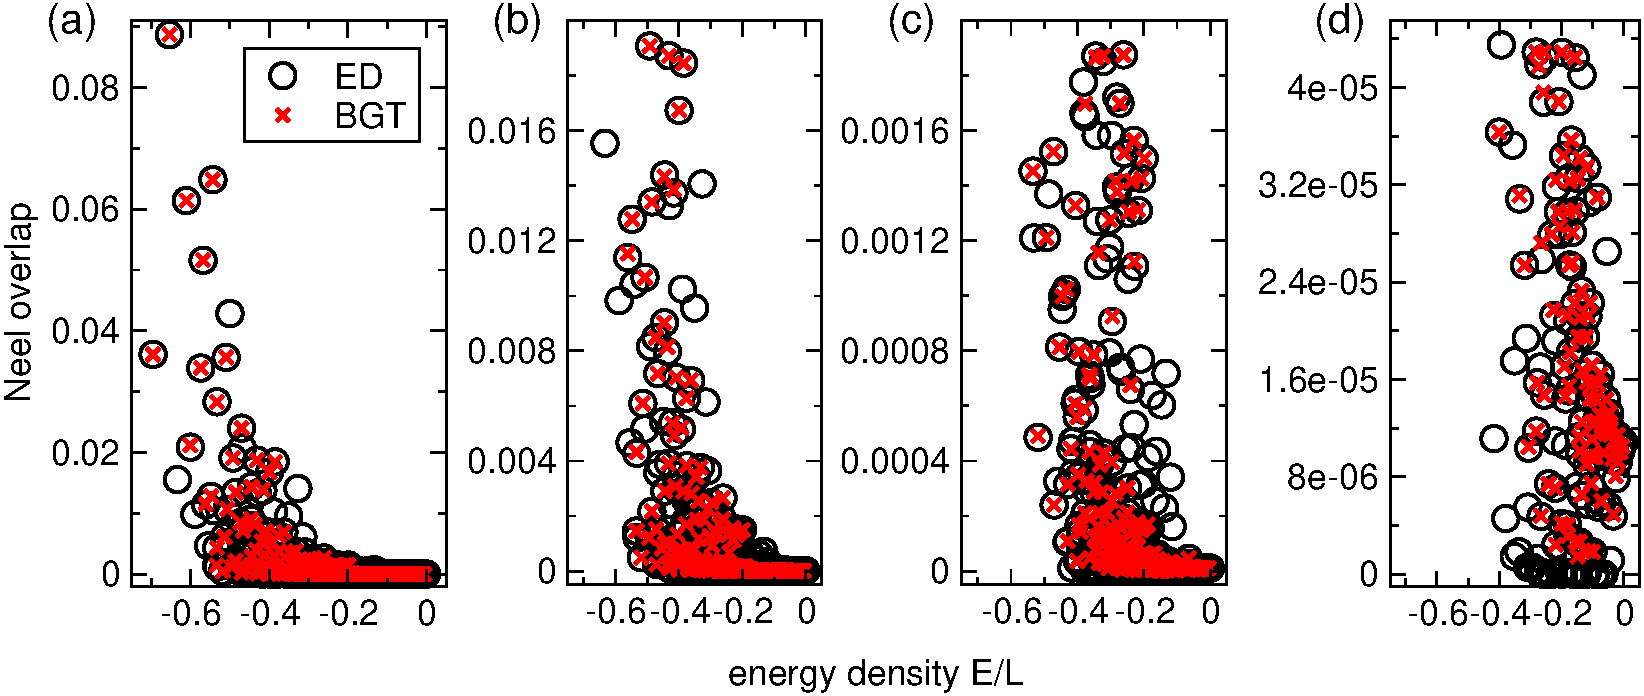
\includegraphics[width=.9\textwidth]{./draft_figs/L20_BT_check}
\end{center}
\caption{ The squared overlap $|\langle N|\lambda\rangle|^2$ between the the 
 Neel state $|N\rangle$ and the eigenstates $|\lambda\rangle$ of the $XXX$ 
 chain with $L=20$ sites. Only non-zero overlaps are shown. In all the panels the 
 $x$-axis shows the eigenstate energy density $E/L$. The circles are the exact 
 diagonalization results for all the non-zero overlaps. The crosses are the Bethe 
 ansatz results obtained using the Bethe-Gaudin-Takahashi equations. The missing 
 crosses correspond to eigenstates containing zero-momentum strings. (a) Overview 
 of all the non-zero overlaps. (b)(c)(d) The same overlaps as in (a) zooming in 
 the regions $[0,0.2]$, $[0,0.020]$, and $[0,4\cdot 10^{-5}]$. The discrepancies 
 between the ED and the Bethe ansatz results are attributed to the string 
 deviations. 
}
\label{fig1-BGT-check}
\end{figure}
%##################################################################

%%%%%%%%%%%%%%%%%%%%%%%%%%%%%%%%%%%%%%%%%%
\begin{table}[h]
\scriptsize
\centering
Bethe states with nonzero N\'eel overlap ($L=12$)\\[1ex]
\begin{tabular}{rrrrrr}
\toprule
String content & $2I_n$ & $q$ & E & $|\langle\lambda|MG\rangle|^2$ (exact) & $|\langle\lambda|MG\rangle|^2$ (BGT) \\[0.3em]
\toprule
\{6,0,0,0,0,0\} &$1_1 3_1 5_1$ & $6$ & $-8.387390917445$ & $0.716615769224$ & $0.716615769224$\\
\midrule
\{2,2,0,0,0,0\} &$1_1 1_2$ & $4$ & $-5.401838225870$ & $0.055624700196$ & $0.05{\color{red}4033366543}$\\  
&$3_1 1_2 $ & & $-4.613929948329$ & $0.005687428810$ & $0.005{\color{red}582983043}$\\
&$5_1 1_2 $ &  & $-3.147465758841$ & $0.002107475934$ & $0.002107{\color{red}086933}$\\
\midrule
\{3,0,1,0,0,0\} &$0_1 2_1 0_3$ & $4$ & $-6.340207488736$ & $0.205891158647$ & -\\
  &$0_1 4_1 0_3$ & & $-5.203653009936$ & $0.038832154450$ & - \\
  &$0_1 6_1 0_3$ & & $-3.788693957250$ & $0.006019410923$ & - \\
\midrule
\{1,0,0,0,1,0\} &$0_1 0_5$ & $2$ & $-2.444293750583$ & $0.000129601311$ & - \\
\midrule
\{0,0,2,0,0,0\} &$1_3$ & $2$ & $-1.111855930538$ & $0.000011727787$ & $0.00001{\color{red}2785580}$\\
\midrule
\{0,1,0,1,0,0\} &$0_2 0_4$ & $2$ &  $-1.560671012472$ & $0.000330572718$ & - \\
\bottomrule
\end{tabular}
\caption{All Bethe states for $L=12$ having nonzero overlap with the zero-momentum Majumdar-Ghosh (MG) 
 state. The first column shows the string content of the Bethe states. The second and third column show 
 $2I_n$, with $I_n$ the BGT quantum numbers identifying the different states, and the number $q$ 
 of independent strings. Due to the parity invariance, we show only the positive quantum numbers. 
 In the second column only the positive BGT numbers are shown. Note that, in 
 contrast to Table~\ref{table:neel} no states with infinite rapidities are present. The fourth column 
 is the Bethe state eigenenergy. Finally, the last two columns show the exact overlap with the MG state 
 and the approximate result obatained using the BGT equations. In the last column Bethe states containing 
 zero-momentum strings are excluded. Deviations from the exact result (digits with different colors) 
 are attributed to the string hypothesis. 
}
\label{table:mg}
\end{table}
%%%%%%%%%%%%%%%%%%%%%%%%%%%%%%%%%%%%%%%%%%

%%%%%%%%%%%%%%%%%%%%%%%%%%%%%%%%%%%%%%%%%%%%%%%%%%%%%%%%%%%%%%%%%%%%%%%%%%%
\subsection{Majumdar-Ghosh overlap}
\label{app-mg}

The overlap between all the Heisenberg chain eigenstates with the Majumdar-Ghosh state are shown in 
Table~\ref{table:mg} for the chain with $L=12$ sites. The conventions on the representation of 
the eigenstates is the same as in Table~\ref{table:neel}. Note that in contrast with the N\'eel 
state, only the eigenstates with zero total spin $S=0$ have non zero overlap, i.e., no eigenstates 
with infinite rapidities are present, which reflect that the Majumdar-Ghosh state is unvariant 
under $SU(2)$ rotations. 


%%%%%%%%%%%%%%%%%%%%%% REFERENCES %%%%%%%%%%%%%%%%%%%%%%%%%%%%%%%%%%%%%%%%%%%%%%%%
\section*{References}
\begin{thebibliography}{99}


%%% EXPERIMENTS
\bibitem{bloch-2008}
I.~Bloch, J.~Dalibard, and W.~Zwerger, Rev.\ Mod.\ Phys.\ {\bf 80},
885 (2008).

\bibitem{greiner-2002}
M.~Greiner, O.~Mandel, T. H\"ansch, and I.~Bloch, Nature (London)
{\bf 419}, 51 (2002).

\bibitem{kinoshita-2006}
T.~Kinoshita, T.~Wenger, and D.~S.~Weiss, Nature (London) {\bf 440},
900 (2008).

\bibitem{hofferberth-2007}
S.~Hofferberth, I.~Lesanovsky, B.~Fischer, T.~Schumm, and J.~Schiedmayer,
Nature (London) {\bf 449}, 324 (2007).

\bibitem{trotzky-2012}
S.~Trotzky, Y.-A.~Chen, A.~Flesch, I.~P.~McCulloch, U.~Schollw\"ock,
J.~Eisert, and I.~Bloch, Nature Phys.\ {\bf 8}, 325 (2012).

\bibitem{gring-2012}
M.~Gring, M.~Kuhnert, T.~Langen, T.~Kitagawa, B.~Rauer, M.~Schreitl,
I.~Mazets, D.~A.~Smith, E.~Demler, and J.~Schmiedmayer, Science {\bf 337},
6100 (2012).

\bibitem{cheneau-2012}
M.~Cheneau, P.~Barmettler, D.~Poletti, M.~Endres, P.~Schaua, T.~Fukuhara,
C.~Gross, I.~Bloch, C.~Kollath, and S.~Kuhr, Nature (London) {\bf 481},
484 (2012).

\bibitem{schneider-2012}
U.~Schneider, L.~Hackeruller, J.~P.~Ronzheimer, S.~Will, S.~Braun, T.~Best,
I.~Bloch, E.~Demler, S.~Mandt, D.~Rasch, and A.~Rosch, Nature\ Phys.\
{\bf 8}, 213 (2012).

\bibitem{kunhert-2013}
M.~Kuhnert, R.~Geiger, T.~Langen, M.~Gring, B.~Rauer,
T.~Kitagawa, E.~Demler, D.~Adu Smith, and J.~Schmiedmayer, Phys.\ Rev.\
Lett.\ {\bf 110}, 090405 (2013).

\bibitem{langen-2013}
T.~Langen, R.~Geiger, M.~Kuhnert, B.~Rauer, and J.~Schmiedmayer,
Nature\ Phys.\ {\bf 9}, 640 (2013).

\bibitem{meinert-2013}
F.~Meinert, M.~J.~Mark, E.~Kirilov, K.~Lauber, P.~Weinmann,
A.~J.~Daley, and H.-C.~Nagerl, Phys.\ Rev.\ Lett.\ {\bf 111},
053003 (2013).

\bibitem{fukuhara-2013}
T.~Fukuhara, A.~Kantian, M.~Endres, M.~Cheneau, P.~Schaua, S.~Hild, C.~Gross,
U.~Schollw\"ock, T.~Giamarchi, I.~Bloch, and S.~Kuhr, Nature\ Phys.\ {\bf 9},
235 (2013).

\bibitem{ronzheimer-2013}
J.~P.~Ronzheimer, M.~Schreiber, S.~Braun, S.~S.~Hodgman, S.~Langer, I.~P.~McCulloch,
F. Heidrich-Meisner, I.~Bloch, and U.~Schneider, Phys.\ Rev.\ Lett.\ {\bf 110},
205301 (2013).

\bibitem{braun-2014}
S.~Braun, M.~Friesdorf, S.~Hodgman, M.~Schreiber, J.~Ronzheimer, A.~Riera, M.~del Rey,
I.~Bloch, J.~Eisert, and U.~Schneider, PNAS {\bf 112}, 3641 (2015).

\bibitem{langen-2015}
T.~Langen, S.~Erne, R.~Geiger, B.~Rauer, T.~Schweigier, M.~Kuhnert, W.~Rohringer,
I.~E.~Mazets, T.~Gasenzer, J.~Schmiedmayer, Science {\bf 348}, 6231 (2015).


%%% QUENCHES
\bibitem{polkovnikov-2011}
A.~Polkovnikov, K.~Sengupta, A~Silva, and M.~Vengalattore, Rev.\ Mod.\ Phys.\
{\bf 83}, 863 (2011).

\bibitem{calabrese-2006}
P.~Calabrese and J.~Cardy, Phys.\ Rev.\ Lett.\ {\bf 96}, 136801 (2006). 

\bibitem{rigol-2007}
M.~Rigol, V.~Dunjko, V.~Yurovsky, and M.~Olshanii, Phys.\ Rev.\ Lett.\ 
{\bf 98}, 050405 (2007). 

\bibitem{calabrese-2007}
P.~Calabrese and J.~Cardy, J.\ Stat.\ Mech.\ (2007) P06008.

\bibitem{kollath-2007}
C.~Kollath, A.~M.~L\"auchli, and E.~Altman, Phys.\ Rev.\ Lett.\ 
{\bf 98}, 180601 (2007).

\bibitem{manmana-2007}
S.~R.~Manmana, S.~Wessel, R.~M.~Noack, and A.~Muramatsu, 
Phys.\ Rev.\ Lett.\ {\bf 98}, 210405 (2007).

\bibitem{rigol-2008}
M.~Rigol, V.~Dunjko, and M.~Olshanii, Nature {\bf 452}, 854 (2008). 

\bibitem{cramer-2008}
M.~Cramer, C.~M.~Dawson, J.~Eisert, and T.~J.~Osborne, Phys.\ Rev.\ 
Lett.\ {\bf 100}, 030602 (2008).

\bibitem{barthel-2008}
T.~Barthel and U.~Schollw\"ock, Phys.\ Rev.\ Lett.\ {\bf 100}, 100601 
(2008). 

\bibitem{kollar-2008}
M.~Kollar and M.~Eckstein, Phys.\ Rev.\ A {\bf 78}, 013626 (2008). 

\bibitem{moeckel-2008}
M.~Moeckel and S.~Kehrein, Phys.\ Rev.\ Lett.\ {\bf 100}, 175702 (2008). 

\bibitem{iucci-2009}
A.~Iucci and M.~A.~Cazalilla, Phys.\ Rev.\ A\ {\bf 80}, 063619 (2009).

\bibitem{rossini-2009}
D.~Rossini, A.~Silva, G.~Mussardo, and G.~E.~Santoro, Phys.\ Rev.\ 
Lett.\ {\bf 102}, 127204 (2009).

\bibitem{barmettler-2009}
P.~Barmettler, M.~Punk, V.~Gritsev, E.~Demler, and E.~Altman, Phys.\ Rev.\ 
Lett.\ {\bf 102}, 130603 (2009).

\bibitem{biroli-2010}
G.~Biroli, C.~Kollath, and A.~M.~L\"auchli, Phys.\ Rev.\ Lett.\ 
{\bf 105}, 250401 (2010). 

\bibitem{rossini-2010}
D.~Rossini, S.~Suzuki, G.~Mussardo, G.~E.~Santoro, and A.~Silva, 
Phys.\ Rev.\ B\ {\bf 82}, 144302 (2010).

\bibitem{fioretto-2010}
D.~Fioretto and G.~Mussardo, New\ J.\ Phys.\ {\bf 12}, 
055015 (2010).

\bibitem{gogolin-2011}
C.~Gogolin, M.~P.~Mueller, and J.~Eisert, Phys.\ Rev.\ Lett.\ 
{\bf 106}, 040401 (2011).

\bibitem{banuls-2011}
M.~C.~Ba\~nuls, J.~I.~Cirac, and M.~B.~Hastings, Phys.\ Rev.\ Lett.\ 
{\bf 106}, 050405 (2011). 

\bibitem{calabrese-2011}
P.~Calabrese, F.~H.~L.~Essler, and M.~Fagotti, Phys.\ Rev.\ Lett.\ {\bf106}, 227203 (2011).

\bibitem{rigol-2011}
M.~Rigol and M.~Fitzpatrick, Phys.\ Rev.\ A {\bf 84}, 033640 (2011).

\bibitem{calabrese-2012}
P.~Calabrese, F.~H.~L.~Essler, and M.~Fagotti, J.\ Stat.\ Mech.\ (2012) P07016.

\bibitem{caux-2012}
J.-S.~Caux and R.~M.~Konik, Phys.\ Rev.\ Lett.\ {\bf 109}, 175301 (2012).

\bibitem{essler-2012}
F.~H.~L.~Essler, S.~Evangelisti, and M.~Fagotti, Phys.\ Rev.\ Lett.\ 
{\bf 109}, 247206 (2012). 

\bibitem{cazalilla-2012}
M.~A.~Cazalilla, A.~Iucci, and M.-C.~Chung, Phys.\ Rev.\ E {\bf 85}, 
011133 (2012). 

\bibitem{mossel-2012a}
J.~Mossel and J.-S.~Caux, New\ J.\ Phys.\ {\bf 14} 075006 (2012).

\bibitem{collura-2013}
M.~Collura, S.~Sotiriadis and P.~Calabrese, Phys.\ Rev.\ Lett.\ {\bf 110}, 245301 (2013)

\bibitem{mussardo-2013}
G.~Mussardo, Phys.\ Rev.\ Lett.\ {\bf 111}, 100401 (2013).

\bibitem{caux-2013}
J.-S.~Caux and F.~H.~L.~Essler, Phys.\ Rev.\ Lett.\ {\bf 110}, 
257203 (2013). 

\bibitem{fagotti-2013}
M.~Fagotti and F.~H.~L.~Essler, Phys.\ Rev.\ B\ {\bf87}, 245107 (2013).

\bibitem{sotiriadis-2014}
S.~Sotiriadis and P.~Calabrese, J.\ Stat.\ Mech.\ (2014) P07024. 

\bibitem{fagotti-2014}
M.~Fagotti, M.~Collura, F.~H.~L.~Essler, and P.~Calabrese, Phys.\ Rev.\ B {\bf 89}, 
125101 (2014).

\bibitem{essler-2014}
F.~H.~L.~Essler, S.~Kehrein, S.~R.~Manmana, and N.~J.~Robinson, Phys.\ Rev.\ B {\bf 89}, 
165104 (2014).

\bibitem{goldstein-2014}
G.~Goldstein and N.~Andrei, arXiv:1405.4224. 

\bibitem{wright-2014}
T.~M.~Wright, M.~Rigol, M.~J.~Davis, and K.~V.~Kheruntsyan, Phys.\ Rev.\ Lett.\ {\bf 113}, 
050601 (2014).

\bibitem{pozsgay-2014}
B.~Pozsgay, M.~Mesty\'an, M.~A.~Werner, M.~Kormos, G.~Zar\'and, and G.~Tak\'acs,
Phys.\ Rev.\ Lett.\ {\bf 113}, 117203 (2014). 

\bibitem{mestyian-2015}
M~Mesty\'an, B.~Pozsgay, G.~Tak\'acs, and M.~A.~Werner, J.\ Stat.\ Mech.\ (2015) 
P04001.

\bibitem{kcc14}
M.~Kormos, M.~Collura, and P.~Calabrese, Phys.\ Rev.\ A {\bf 89}, 013609 
(2014).

\bibitem{kcc14a}
P.~P.~Mazza, M.\ Collura, M.\ Kormos, and P.\ Calabrese, J.\ Stat.\ Mech.\  
(2014) P11016.

\bibitem{mossel-2012}
J.~Mossel and J.-S.~Caux, J.\ Phys.\ A:\ Math.\ Theor.\ {\bf 45}, 
255001 (2012). 

\bibitem{pozsgay-2013}
B.~Pozsgay, J.\ Stat.\ Mech.\ (2013) P07003. 

\bibitem{calabrese-2014}
P.~Calabrese and P.~Le Doussal, J.\ Stat.\ Mech.\ (2014) P05004. 

\bibitem{alba-2015}
V.~Alba, arXiv:1507.06994.

\bibitem{calabrese-2007}
P.~Calabrese and J.-S.~Caux, Phys.\ Rev.\ Lett.\ {\bf 98}, 150403 (2007).

\bibitem{calabrese-2007-a}
P.~Calabrese and J.-S.~Caux, J.\ Stat.\ Mech.\ P08032 (2007).

\bibitem{de-nardis-2014}
J.~De Nardis, B.~Wouters, M.~Brockmann, and J.-S.~Caux, Phys.\ Rev.\ A {\bf 89}, 
033601 (2014). 

\bibitem{pozsgay-2014}
B.~Pozsgay, M.~Mesty\'an, M.~A.~Werner, M.~Kormos, G.~Zar\'and, and G.~Tak\'acs,
Phys.\ Rev.\ Lett.\ {\bf 113}, 117203 (2014). 

\bibitem{wouters-2014}
B.~Wouters, M.~Brockmann, J.~De~Nardis, D.~Fioretto, M.~Rigol, and J.-S.~Caux, 
Phys.\ Rev.\ Lett.\ {\bf 113}, 117202 (2014). 

\bibitem{brockmann-2014a}
M.~Brockmann, B.~Wouters, D.~Fioretto, J.~De Nardis, R.~Vlijm, and J.-S.~Caux, 
J.\ Stat.\ Mech.\ (2014) P12009. 

\bibitem{mazza-2015}
P.~P.~Mazza, J.-M.~St\'ephan, E.~Canovi, V.~Alba, M.~Brockmann, and M.~Haque, 
arXiv:1509.04666.

\bibitem{fagotti-2013}
M.~Fagotti and F.~H.~Essler, J.\ Stat.\ Mech.\ (2013) P07012. 

%%% BETHE ANSATZ
\bibitem{bethe-1931}
H.~Bethe, Z.\ Phys.\ {\bf 71}, 205 (1931). 

\bibitem{kor-book}
V.~E.~Korepin, N.~M.~Bogoliubov, and A.~G.~Izergin, \emph{Quantum 
Inverse Scattering Methods and Correlation Functions}, Cambridge 
University Press, Cambridge, 1997. 

\bibitem{takahashi-1971} 
M.~Takahashi, Prog.\ Theor.\ Phys.\ {\bf 46}, 401 (1971). 

\bibitem{taka-book}
M.~Takahashi, {\it Thermodynamics of one-dimensional solvable models}, 
Cambridge University Press, Cambridge, 1999. 

\bibitem{gu-2005}
S.-J.~Gu, N.~M.~R.~Peres, Y.-Q.~Li, Eur.\ Phys.\ J.\ B {\bf 48}, 157 (2005). 

\bibitem{faddeev-1996}
L.~D.~Faddeev, arXiv:9605187.

\bibitem{yang-1969}
C.~N.~Yang and C.~P.~Yang, J.\ Math.\ Phys. {\bf 10}, 1115 (1969).

%%%CHARGES
\bibitem{grabowski-1995}
M.~P.~Grabowski and P.~Mathieu, Ann.\ Phys.\ N.Y. {\bf 243}, 
299 (1995). 

\bibitem{prosen-2014}
T.~Prosen, Nucl.\ Phys.\ B\ {\bf 886}, (2014) 1177.

\bibitem{pereira-2014}
R.~G.~Pereira, V.~Pasquier, J.~Sirker, and I.~Affleck, J.\ Stat.\ Mech.\ 
(2014) P09037. 

\bibitem{ilievski-2015}
E.~Ilievski, M.~Medejak, and T.~Prosen, arXiv:1506.05049.

\bibitem{ilievski-2015a}
E.~Ilieveski, J.~De~Nardis, B.~Wouters, J.-S.~Caux, F.~H.~Essler, and T.~Prosen, 
arXiv:1507.02993. 

\bibitem{essler-2015}
F.~H.~L.~Essler, G.~Mussardo, and M.~Panfil, Phys.\ Rev.\ A {\bf 91}, 051602 (2015). 

\bibitem{cardy-2015}
J.~Cardy,  arXiv:1507.07266.


%%%MONTE CARLO
\bibitem{landau-binder}
D.~P.~Landau and K.~Binder, \emph{A Guide to Monte Carlo Simulations in 
Statistical Physics}, Cambridge University Press, Cambridge, 2000.

\bibitem{quenouille-1949} 
M.~H.~Quenouille, Ann.\ Math.\ Statist.\ {\bf 20}, 355 (1949).

\bibitem{wolff-2004} 
U.~Wolff, Comput.\ Phys.\ Comm.\ {\bf 156}, 143 (2004). 

%%% OVERLAPS
\bibitem{brockmann-2014}
M.~Brockmann, J.~De~Nardis, B.~Wouters, and J.-S.~Caux, J.\ Phys.\ A:\ 
Math.\ Theor. {\bf 47}, 345003 (2014). 

\bibitem{brockmann-2014c}
M.~Brockmann, J.~De~Nardis, B.~Wouters, and J.-S.~Caux, J.\ Phys.\ A:\ 
Math.\ Theor. {\bf 47}, 145003 (2014). 

\bibitem{brockmann-2014b}
M.~Brockmann, J.\ Stat.\ Mech.\ (2014) P05006. 

\bibitem{pozsgay-2014a}
B.~Pozsgay, J.\ Stat.\ Mech.\ (2014) P06011. 

\bibitem{piroli-2014}
L.~Piroli and P.~Calabrese, J.\ Phys.\ A {\bf 47}, 385003 (2014). 

%%%ETH
\bibitem{alba-2015a}
V.~Alba, Phys.\ Rev.\ B {\bf 91}, 155123 (2015). 

\bibitem{ikeda-2013}
T.~N.~Ikeda, Y.~Watanabe, and M.~Ueda, Phys.\ Rev.\ E {\bf 87}, 012125 (2013). 

\end{thebibliography}


\end{document}


